\documentclass[11pt,a4paper]{article}

% Image mode: pdf.
% Image paths stay relative. In PDF mode, place same-basename PDF conversions
% of the chapter SVG files in the assets/ directory beside this source.

\usepackage{iftex}
\ifPDFTeX
  \PackageError{handout}{This template requires XeTeX or Tectonic}{Compile with xelatex or tectonic.}
\fi

\usepackage[a4paper,top=18mm,bottom=20mm,left=20mm,right=20mm,headsep=6mm]{geometry}
\usepackage{fontspec}
\usepackage{xeCJK}
\usepackage{amsmath}
\usepackage{unicode-math}

% Font settings are intentionally visible in the generated .tex file.
% These defaults target the macOS machine used for the released PDF.
% Change the family names when compiling on another system.
\setmainfont{Songti TC}
\setsansfont{Heiti TC}
\setmonofont{Menlo}
\setCJKmainfont{Songti TC}
\setCJKsansfont{Heiti TC}
\setCJKmonofont{Heiti TC}
\setmathfont{STIX Two Math}
\XeTeXlinebreaklocale "zh"
\XeTeXlinebreakskip=0pt plus 1pt

\usepackage{xcolor}
\definecolor{HandoutBlue}{HTML}{215A91}
\definecolor{HandoutBlueLight}{HTML}{EEF5FC}
\definecolor{HandoutGreen}{HTML}{39715A}
\definecolor{HandoutGreenLight}{HTML}{EFF8F3}
\definecolor{HandoutGold}{HTML}{8A641C}
\definecolor{HandoutGoldLight}{HTML}{FFF8E8}
\definecolor{HandoutInk}{HTML}{253142}
\definecolor{HandoutMuted}{HTML}{667085}

\usepackage{graphicx}
\makeatletter
% Pandoc 3 emits an accessibility `alt` key for raster/PDF images. Older
% graphicx releases do not know that key, so accept it without changing layout.
\@ifundefined{KV@Gin@alt}{\define@key{Gin}{alt}{}}{}
\newsavebox\pandoc@box
\newcommand*\pandocbounded[1]{%
  \sbox\pandoc@box{#1}%
  \Gscale@div\@tempa{\textheight}{\dimexpr\ht\pandoc@box+\dp\pandoc@box\relax}%
  \Gscale@div\@tempb{\linewidth}{\wd\pandoc@box}%
  \ifdim\@tempb\p@<\@tempa\p@\let\@tempa\@tempb\fi
  \ifdim\@tempa\p@<\p@\scalebox{\@tempa}{\usebox\pandoc@box}%
  \else\usebox{\pandoc@box}%
  \fi
}
\makeatother
\usepackage{float}
\floatplacement{figure}{H}
% Pandoc uses LTcaptype=none for uncaptioned longtables. The caption package
% expects that name to exist as a counter even though it is never displayed.
\newcounter{none}
\usepackage{caption}
\captionsetup[figure]{labelformat=empty,labelsep=none,font=small}

\usepackage{booktabs,longtable,array,calc}
\usepackage{etoolbox}
\makeatletter
\patchcmd\longtable{\par}{\if@noskipsec\mbox{}\fi\par}{}{}
\makeatother

\usepackage[most]{tcolorbox}
\tcbuselibrary{breakable,skins}
\newtcolorbox{HandoutLearningMap}{
  enhanced,breakable,colback=HandoutBlueLight,colframe=HandoutBlue,
  boxrule=0.8pt,arc=1.5mm,left=3mm,right=3mm,top=2mm,bottom=2mm,
  before skip=8pt,after skip=10pt
}
\newtcolorbox{HandoutWorkedExample}{
  enhanced,breakable,colback=HandoutGreenLight,colframe=HandoutGreen,
  boxrule=0.65pt,arc=1.5mm,left=3mm,right=3mm,top=2mm,bottom=2mm,
  before skip=8pt,after skip=10pt
}
\newtcolorbox{HandoutSelfCheck}{
  enhanced,breakable,colback=HandoutGoldLight,colframe=HandoutGold,
  boxrule=0.65pt,arc=1.5mm,left=3mm,right=3mm,top=2mm,bottom=2mm,
  before skip=8pt,after skip=10pt
}

\usepackage{titlesec}
\titleformat{\section}{\sffamily\bfseries\Large\color{HandoutBlue}}{}{0pt}{}
\titleformat{\subsection}{\sffamily\bfseries\large\color{HandoutInk}}{}{0pt}{}
\titleformat{\subsubsection}{\sffamily\bfseries\normalsize\color{HandoutInk}}{}{0pt}{}
\titlespacing*{\section}{0pt}{1.4em}{0.55em}
\titlespacing*{\subsection}{0pt}{1.15em}{0.45em}
\titlespacing*{\subsubsection}{0pt}{0.9em}{0.35em}
\setcounter{secnumdepth}{-\maxdimen}

\usepackage{hyperref}
\usepackage{bookmark}
\IfFileExists{xurl.sty}{\usepackage{xurl}}{}
\urlstyle{same}
\hypersetup{
  colorlinks=true,
  linkcolor=HandoutBlue,
  urlcolor=HandoutBlue,
  citecolor=HandoutBlue,
  pdftitle={選化III-2 酸鹼反應},
  pdfsubject={化學},
  pdfcreator={Pandoc with the HighSchooContent LaTeX template}
}

\setlength{\parindent}{0pt}
\setlength{\parskip}{0.55em plus 0.15em minus 0.1em}
\setlength{\emergencystretch}{3em}
\setlength{\LTpre}{0.5em}
\setlength{\LTpost}{0.5em}
\renewcommand{\arraystretch}{1.18}
\providecommand{\tightlist}{%
  \setlength{\itemsep}{0pt}\setlength{\parskip}{0pt}}
\pagestyle{plain}


\begin{document}

\begin{tcolorbox}[
  enhanced,colback=white,colframe=HandoutBlue,boxrule=1.1pt,arc=2mm,
  borderline west={3pt}{0pt}{HandoutBlue},left=5mm,right=4mm,top=4mm,bottom=4mm
]
{\sffamily\small\bfseries\color{HandoutBlue}學生講義}\par
{\sffamily\bfseries\LARGE\color{HandoutInk}選化III-2 酸鹼反應}\par
\vspace{0.35em}{\large 由質子轉移與解離平衡，定量連結水解、緩衝、滴定曲線與酸鹼分析}\par
\vspace{0.45em}{\small\color{HandoutMuted}%
科目：化學
\quad 課程：普通高中選修化學 III
\quad 版本：學生版｜核心＋理解
\quad 校訂：2026-08-29
}\par
\vspace{0.25em}{\small\color{HandoutMuted}範圍：現行選修化學 III 第二章主線；涵蓋酸鹼命名、布－洛酸鹼、Kw／Ka／Kb、同離子與多質子酸、鹽類水解、緩衝溶液、酸鹼滴定與滴定曲線}\par
\end{tcolorbox}


酸鹼反應把一個質子從供體移到受體；解離常數量化這個轉移在水中的平衡位置。沿著同一套粒子與電荷帳，可以計算弱酸、弱鹼與鹽類水溶液的 pH，設計能穩定 pH 的緩衝液，再由滴定曲線把未知濃度、酸鹼強弱與指示劑選擇連成可量測的分析方法。實際用途包括水質監測、食品酸度分析、藥品配方與化學製程的 pH 控制。

\begin{HandoutLearningMap}

\subsection{本章問題與能力}\label{ux672cux7ae0ux554fux984cux8207ux80fdux529b}

\begin{enumerate}
\def\labelenumi{\arabic{enumi}.}
\tightlist
\item
  如何由化學式命名酸、鹼與鹽，並判斷真正可解離的質子數？
\item
  如何辨認布－洛酸鹼、共軛酸鹼對與質子轉移方向？
\item
  如何用 \(K_w\)、\(K_a\)、\(K_b\)、質量平衡與電荷平衡求水溶液組成？
\item
  同離子、多質子酸與鹽類水解如何改變主要物種與 pH？
\item
  緩衝液如何吸收少量強酸、強鹼，目標 pH 與緩衝容量如何設計？
\item
  如何由滴定裝置、化學計量、滴定曲線與指示劑範圍測定未知樣品？
\end{enumerate}

\end{HandoutLearningMap}

本章以高中常用的稀水溶液模型計算，將離子活度近似為體積莫耳濃度。溫度、離子強度或濃度很高時，精密分析需改用活度與儀器校正；題目若指定溫度或 \(K_w\)，便使用該條件的數值。

\section{1. 酸、鹼的化學式、命名與可解離質子}\label{ux9178ux9e7cux7684ux5316ux5b78ux5f0fux547dux540dux8207ux53efux89e3ux96e2ux8ceaux5b50}

\subsection{1.1 無氧酸、含氧酸與金屬氫氧化物}\label{ux7121ux6c27ux9178ux542bux6c27ux9178ux8207ux91d1ux5c6cux6c2bux6c27ux5316ux7269}

無氧酸由氫與不含氧的陰離子組成。氣態分子與水溶液需連同狀態辨認：

{\def\LTcaptype{none} % do not increment counter
\begin{longtable}[]{@{}ll@{}}
\toprule\noalign{}
化學式 & 名稱 \\
\midrule\noalign{}
\endhead
\bottomrule\noalign{}
\endlastfoot
\(HCl(g)\) & 氯化氫 \\
\(HCl(aq)\) & 氫氯酸，常稱鹽酸 \\
\(H_2S(aq)\) & 氫硫酸 \\
\(HCN(aq)\) & 氫氰酸 \\
\end{longtable}
}

同一中心原子的含氧酸可依氧原子數區分。氯的含氧酸形成一組可直接比較的系列：

{\def\LTcaptype{none} % do not increment counter
\begin{longtable}[]{@{}lll@{}}
\toprule\noalign{}
化學式 & 名稱 & 共軛鹼 \\
\midrule\noalign{}
\endhead
\bottomrule\noalign{}
\endlastfoot
\(HClO_4\) & 過氯酸 & \(ClO_4^-\) \\
\(HClO_3\) & 氯酸 & \(ClO_3^-\) \\
\(HClO_2\) & 亞氯酸 & \(ClO_2^-\) \\
\(HClO\) & 次氯酸 & \(ClO^-\) \\
\end{longtable}
}

金屬氫氧化物命名為「氫氧化某」。金屬有多種常見氧化數時，可在名稱後標示氧化數，例如 \(Fe(OH)_2\) 為氫氧化鐵（2），\(Fe(OH)_3\) 為氫氧化鐵（3）。

\subsection{1.2 可解離質子由結構決定}\label{ux53efux89e3ux96e2ux8ceaux5b50ux7531ux7d50ux69cbux6c7aux5b9a}

分子式中的氫原子數不必等於可解離質子數。磷的三種含氧酸可用結構中的 \(O-H\) 鍵判斷：

\begin{itemize}
\tightlist
\item
  \(H_3PO_4\) 有三個 \(O-H\)，是三質子酸。
\item
  \(H_3PO_3\) 的結構可寫為 \(HPO(OH)_2\)，有兩個 \(O-H\)，是二質子酸。
\item
  \(H_3PO_2\) 的結構可寫為 \(H_2PO(OH)\)，有一個 \(O-H\)，是單質子酸。
\end{itemize}

這項判斷同時決定中和計量。若 \(1\) mol 酸在指定反應中完整釋出 \(a\) mol \(H^+\)，與強鹼完全反應便需要 \(a\) mol \(OH^-\)。

含氯漂白水中的 \(ClO^-\) 遇酸會生成有毒氯氣：

\[
ClO^-+Cl^-+2H^+\rightarrow Cl_2+H_2O.
\]

反應前後都有兩個氯、兩個氫、一個氧，總電荷均為零。含氯漂白水應依產品標示單獨使用並保持通風；酸性清潔劑與含氨清潔劑都需分開存放與使用。

\begin{HandoutWorkedExample}

\subsection{示範 1｜由化學式命名並判斷類型}\label{ux793aux7bc4-1ux7531ux5316ux5b78ux5f0fux547dux540dux4e26ux5224ux65b7ux985eux578b}

依序處理 \(HMnO_4\)、\(HNO_2\)、\(Ca(OH)_2\)、\(Fe(OH)_3\)。

\begin{enumerate}
\def\labelenumi{\arabic{enumi}.}
\tightlist
\item
  \(HMnO_4\) 的酸根是過錳酸根 \(MnO_4^-\)，名稱為過錳酸。
\item
  \(HNO_2\) 的酸根是亞硝酸根 \(NO_2^-\)，名稱為亞硝酸。
\item
  \(Ca(OH)_2\) 含 \(Ca^{2+}\) 與兩個 \(OH^-\)，名稱為氫氧化鈣。
\item
  \(Fe(OH)_3\) 中鐵的氧化數為 \(+3\)，名稱為氫氧化鐵（3）。
\end{enumerate}

名稱中的前綴、酸根與金屬氧化數都由化學式的組成與電荷決定。

\end{HandoutWorkedExample}

\begin{HandoutWorkedExample}

\subsection{示範 2｜結構、質子數與中和計量}\label{ux793aux7bc4-2ux7d50ux69cbux8ceaux5b50ux6578ux8207ux4e2dux548cux8a08ux91cf}

\(0.0200\) mol \(H_3PO_3\) 與足量 \(NaOH\) 完全反應。\(H_3PO_3=HPO(OH)_2\) 有兩個可解離的 \(O-H\)，因此

\[
H_3PO_3+2NaOH\rightarrow Na_2HPO_3+2H_2O.
\]

所需 \(NaOH\) 為

\[
n_{NaOH}=2(0.0200)=0.0400\ \mathrm{mol}.
\]

產物 \(Na_2HPO_3\) 中仍有一個直接連在磷上的氫；該氫不計入本反應的可解離質子。

\end{HandoutWorkedExample}

酸鹼命名直接服務藥品標示、清潔劑相容性與滴定計量。辨認 \(HClO\)、\(ClO^-\) 與 \(HCl\) 的名稱和粒子形式，便能由反應式追蹤漂白水在不同 pH 下的物種與危害。

\subsection{分節練習 1}\label{ux5206ux7bc0ux7df4ux7fd2-1}

\begin{enumerate}
\def\labelenumi{\arabic{enumi}.}
\tightlist
\item
  寫出 \(HCN(aq)\)、\(HClO_2\)、\(Fe(OH)_2\)、\(H_2MnO_4\) 的中文名稱。
\item
  寫出過氯酸、亞硫酸、氫氧化鋁、氫氧化銅（2）的化學式。
\item
  判斷 \(H_3PO_4\)、\(H_3PO_3\)、\(H_3PO_2\) 的可解離質子數；各取 \(0.0100\) mol 與強鹼完全反應時，所需 \(OH^-\) 各為多少 mol？
\item
  將漂白水酸化產生氯氣的淨離子反應式逐項檢查原子數與總電荷。
\end{enumerate}

\subsection{分節練習 1 解析}\label{ux5206ux7bc0ux7df4ux7fd2-1-ux89e3ux6790}

\begin{enumerate}
\def\labelenumi{\arabic{enumi}.}
\tightlist
\item
  \(HCN(aq)\)：氫氰酸；\(HClO_2\)：亞氯酸；\(Fe(OH)_2\)：氫氧化鐵（2）；\(H_2MnO_4\)：錳酸。
\item
  過氯酸 \(HClO_4\)；亞硫酸 \(H_2SO_3\)；氫氧化鋁 \(Al(OH)_3\)；氫氧化銅（2）\(Cu(OH)_2\)。
\item
  可解離質子數依序為 \(3,2,1\)，所以需要的 \(OH^-\) 依序為 \(0.0300\)、\(0.0200\)、\(0.0100\) mol。
\item
  \[
  ClO^-+Cl^-+2H^+\rightarrow Cl_2+H_2O.
  \]
  左側有 \(Cl_2H_2O_1\)，右側相同；左側電荷為 \(-1-1+2=0\)，右側中性，原子與電荷均守恆。
\end{enumerate}

\section{2. 布－洛酸鹼、共軛對與反應方向}\label{ux5e03ux6d1bux9178ux9e7cux5171ux8edbux5c0dux8207ux53cdux61c9ux65b9ux5411}

\subsection{2.1 酸鹼角色由質子轉移決定}\label{ux9178ux9e7cux89d2ux8272ux7531ux8ceaux5b50ux8f49ux79fbux6c7aux5b9a}

布－洛酸是在一個反應步驟中提供質子 \(H^+\) 的物種；布－洛鹼是接受質子的物種：

\[
\text{酸}_1+\text{鹼}_2\rightleftharpoons\text{鹼}_1+\text{酸}_2.
\]

酸失去一個 \(H^+\) 後成為共軛鹼；鹼接受一個 \(H^+\) 後成為共軛酸。每組共軛酸鹼對只差一個 \(H^+\)。

\begin{figure}
\centering
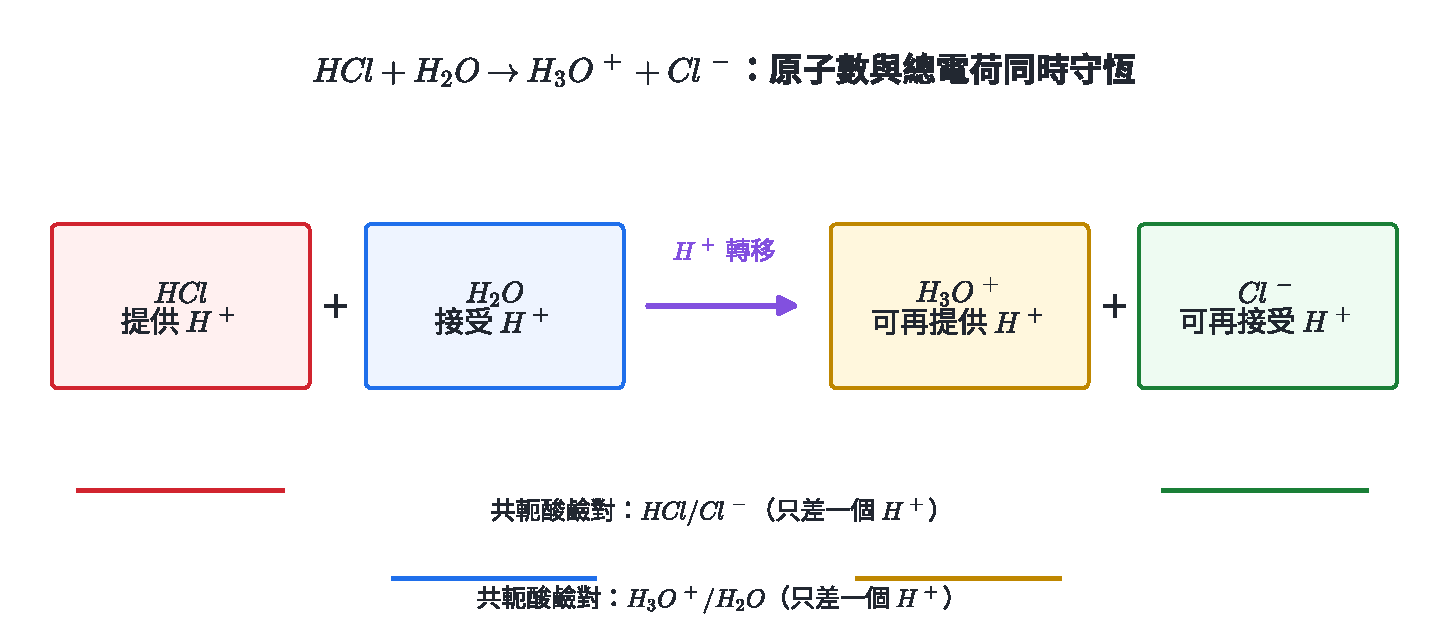
\includegraphics[width=0.96\linewidth,height=\textheight,keepaspectratio,alt={圖 1｜沿箭頭追蹤 HCl 把一個質子交給水；上下連線標出兩組只差一個質子的共軛酸鹼對。}]{assets/選化III-2-質子轉移與共軛對.pdf}
\caption{圖 1｜沿箭頭追蹤 HCl 把一個質子交給水；上下連線標出兩組只差一個質子的共軛酸鹼對。}
\end{figure}

水可依反應對象扮演兩種角色：

\[
HCl+H_2O\rightarrow H_3O^++Cl^- \qquad (H_2O\text{ 接受 }H^+),
\]

\[
NH_3+H_2O\rightleftharpoons NH_4^++OH^- \qquad (H_2O\text{ 提供 }H^+).
\]

能提供也能接受質子的物種稱為兩性物種，例如 \(H_2O\)、\(HCO_3^-\)、\(H_2PO_4^-\)。

\subsection{2.2 反應偏向較弱酸與較弱鹼}\label{ux53cdux61c9ux504fux5411ux8f03ux5f31ux9178ux8207ux8f03ux5f31ux9e7c}

以共軛酸的 \(pK_a\) 比較質子轉移：

\[
HA+B\rightleftharpoons A^-+BH^+,
\]

其平衡常數可近似寫成

\[
K\approx\frac{K_a(HA)}{K_a(BH^+)}
=10^{pK_a(BH^+)-pK_a(HA)}.
\]

\(K>1\) 表示右側較有利。等價地說，平衡偏向酸、鹼都較弱的一側。

\begin{figure}
\centering
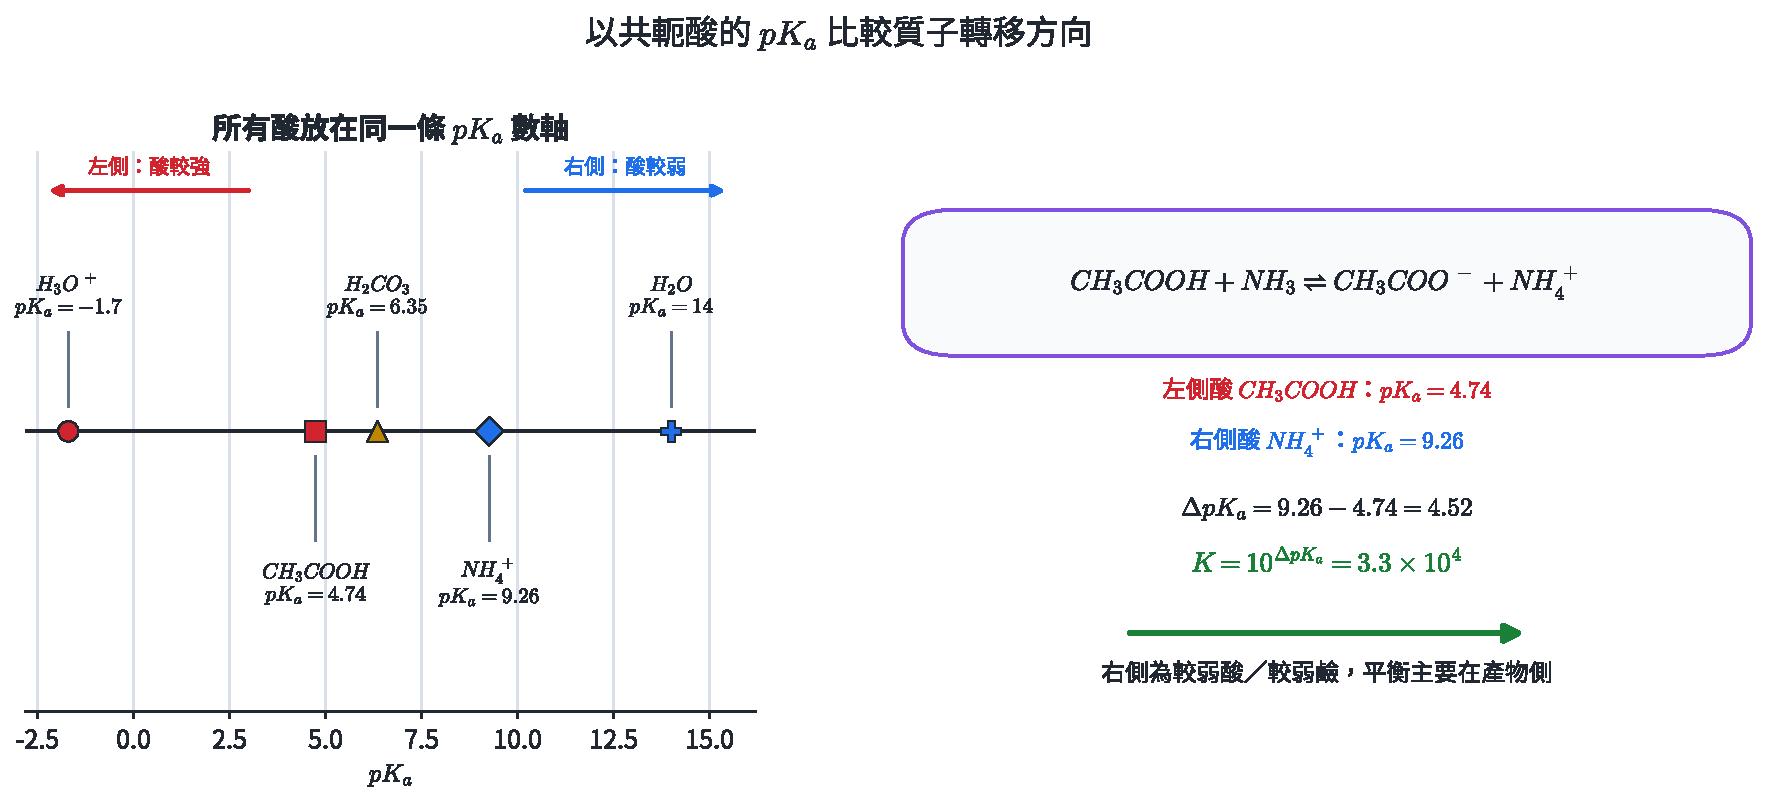
\includegraphics[width=0.97\linewidth,height=\textheight,keepaspectratio,alt={圖 2｜左圖把五種酸放在同一條 pK\_a 數軸；右圖由左右兩側酸的 \textbackslash Delta pK\_a 算得 K=3.3\textbackslash times10\^{}4，因此平衡主要在較弱酸與較弱鹼所在的產物側。}]{assets/選化III-2-酸鹼強度與反應方向.pdf}
\caption{圖 2｜左圖把五種酸放在同一條 \(pK_a\) 數軸；右圖由左右兩側酸的 \(\Delta pK_a\) 算得 \(K=3.3\times10^4\)，因此平衡主要在較弱酸與較弱鹼所在的產物側。}
\end{figure}

\begin{HandoutWorkedExample}

\subsection{示範 3｜辨認兩組共軛酸鹼對}\label{ux793aux7bc4-3ux8fa8ux8a8dux5169ux7d44ux5171ux8edbux9178ux9e7cux5c0d}

考慮

\[
H_2PO_4^-+NH_3\rightleftharpoons HPO_4^{2-}+NH_4^+.
\]

\(H_2PO_4^-\) 失去一個 \(H^+\)，所以是酸；\(HPO_4^{2-}\) 是其共軛鹼。\(NH_3\) 接受一個 \(H^+\)，所以是鹼；\(NH_4^+\) 是其共軛酸。

兩組共軛對為

\[
H_2PO_4^-/HPO_4^{2-},\qquad NH_4^+/NH_3.
\]

原子與電荷檢查：左側總電荷 \(-1\)，右側 \(-2+1=-1\)。

\end{HandoutWorkedExample}

\begin{HandoutWorkedExample}

\subsection{\texorpdfstring{示範 4｜由 \(pK_a\) 求反應方向}{示範 4｜由 pK\_a 求反應方向}}\label{ux793aux7bc4-4ux7531-pk_a-ux6c42ux53cdux61c9ux65b9ux5411}

已知 \(pK_a(CH_3COOH)=4.74\)、\(pK_a(NH_4^+)=9.26\)：

\[
CH_3COOH+NH_3\rightleftharpoons CH_3COO^-+NH_4^+.
\]

\[
K\approx10^{9.26-4.74}=3.3\times10^4.
\]

\(K\) 遠大於 \(1\)，所以主要形成 \(CH_3COO^-\) 與 \(NH_4^+\)。這個結果可用於混合前先完成酸鹼計量，再處理剩餘物種的平衡。

\end{HandoutWorkedExample}

布－洛模型可分析水處理、蛋白質側鏈、藥物鹽型與緩衝系統中的質子流向。它直接描述質子轉移；涉及電子對受體而沒有質子轉移的路易斯酸鹼反應，需使用更廣的模型。

\subsection{分節練習 2}\label{ux5206ux7bc0ux7df4ux7fd2-2}

\begin{enumerate}
\def\labelenumi{\arabic{enumi}.}
\tightlist
\item
  在 \(HCO_3^-+H_2O\rightleftharpoons H_2CO_3+OH^-\) 中，標出酸、鹼及兩組共軛酸鹼對。
\item
  分別寫出 \(HCO_3^-\) 接受 \(H^+\) 與提供 \(H^+\) 的反應，據此說明其兩性。
\item
  已知 \(pK_a(HF)=3.17\)、\(pK_a(CH_3COOH)=4.74\)。估算
  \(HF+CH_3COO^-\rightleftharpoons F^-+CH_3COOH\) 的 \(K\) 與主要方向。
\item
  已知 \(pK_a(NH_4^+)=9.26\)、\(pK_a(CH_3COOH)=4.74\)。判斷
  \(NH_4^++CH_3COO^-\rightleftharpoons NH_3+CH_3COOH\) 的主要方向。
\end{enumerate}

\subsection{分節練習 2 解析}\label{ux5206ux7bc0ux7df4ux7fd2-2-ux89e3ux6790}

\begin{enumerate}
\def\labelenumi{\arabic{enumi}.}
\tightlist
\item
  \(HCO_3^-\) 接受質子，是鹼；\(H_2O\) 提供質子，是酸。共軛對為 \(H_2CO_3/HCO_3^-\) 與 \(H_2O/OH^-\)。
\item
  接受質子：
  \[
  HCO_3^-+H^+\rightarrow H_2CO_3.
  \]
  提供質子：
  \[
  HCO_3^-\rightleftharpoons H^++CO_3^{2-}.
  \]
  它在不同反應中可接受或提供質子，因此具兩性。
\item
  \[
  K\approx10^{4.74-3.17}=3.7\times10^1.
  \]
  反應主要向右，形成較弱酸 \(CH_3COOH\) 與較弱鹼 \(F^-\)。
\item
  \[
   K\approx10^{4.74-9.26}=3.0\times10^{-5}.
   \]
  右向反應不利，主要物種留在左側。
\end{enumerate}

\section{3. 水的離子積、pH 與溫度}\label{ux6c34ux7684ux96e2ux5b50ux7a4dph-ux8207ux6eabux5ea6}

\subsection{\texorpdfstring{3.1 水的自解離與 \(K_w\)}{3.1 水的自解離與 K\_w}}\label{ux6c34ux7684ux81eaux89e3ux96e2ux8207-k_w}

水分子之間可發生質子轉移：

\[
2H_2O(l)\rightleftharpoons H_3O^+(aq)+OH^-(aq).
\]

高中計算常以 \(H^+\) 簡寫 \(H_3O^+\)。定溫下，

\[
K_w=[H^+][OH^-].
\]

酸鹼對數尺度定義為

\[
pH=-\log[H^+],\qquad pOH=-\log[OH^-],\qquad pK_w=-\log K_w,
\]

所以

\[
pH+pOH=pK_w.
\]

中性條件是 \([H^+]=[OH^-]=\sqrt{K_w}\)，因此中性 pH 為 \(\tfrac12pK_w\)。在 \(25\,^\circ\mathrm C\)，\(K_w=1.0\times10^{-14}\)，中性 pH 才恰為 \(7.00\)。

\begin{figure}
\centering
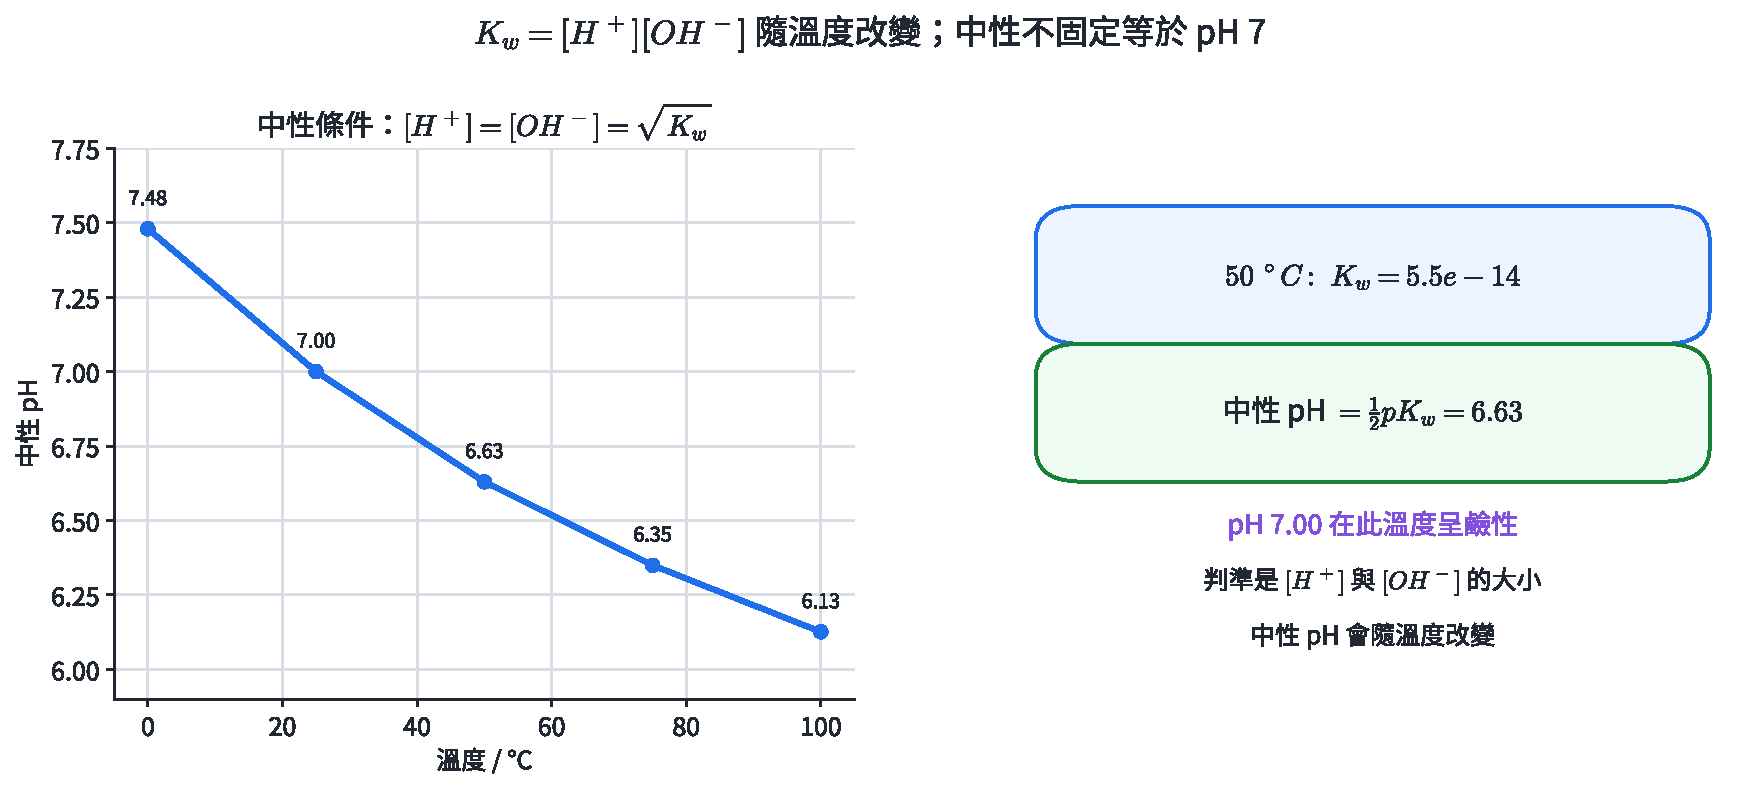
\includegraphics[width=0.97\linewidth,height=\textheight,keepaspectratio,alt={圖 3｜左圖由不同溫度的 Kw 算出中性 pH；右圖以 50 °C 說明 pH 7 相對於中性點的位置。}]{assets/選化III-2-Kw溫度與中性pH.pdf}
\caption{圖 3｜左圖由不同溫度的 Kw 算出中性 pH；右圖以 50 °C 說明 pH 7 相對於中性點的位置。}
\end{figure}

\subsection{3.2 強酸、強鹼與濃度邊界}\label{ux5f37ux9178ux5f37ux9e7cux8207ux6fc3ux5ea6ux908aux754c}

一般濃度的強單質子酸近乎完全解離，可取 \([H^+]\approx C_a\)；強一元鹼可取 \([OH^-]\approx C_b\)。多元強鹼需乘化學計量係數，例如

\[
[OH^-]\approx2C_{Ba(OH)_2}.
\]

當形式濃度接近純水自解離提供的 \([H^+]\) 或 \([OH^-]\) 時，水的貢獻不可省略；本章題目若涉及此區域，會提供或要求完整電荷平衡。

\begin{HandoutWorkedExample}

\subsection{示範 5｜溫度改變時判斷中性與酸鹼}\label{ux793aux7bc4-5ux6eabux5ea6ux6539ux8b8aux6642ux5224ux65b7ux4e2dux6027ux8207ux9178ux9e7c}

\(50\,^\circ\mathrm C\) 時 \(K_w=5.5\times10^{-14}\)。

\[
pK_w=-\log(5.5\times10^{-14})=13.26,
\]

\[
pH_{\mathrm{neutral}}=\frac{13.26}{2}=6.63.
\]

某溶液在此溫度的 pH 為 \(7.00\)，則

\[
pOH=13.26-7.00=6.26.
\]

\(pH>pOH\)，等價於 \([OH^-]>[H^+]\)，所以溶液呈鹼性。

\end{HandoutWorkedExample}

\begin{HandoutWorkedExample}

\subsection{示範 6｜由強鹼質量求 pH}\label{ux793aux7bc4-6ux7531ux5f37ux9e7cux8ceaux91cfux6c42-ph}

在 \(25\,^\circ\mathrm C\)，將 \(0.400\) g \(NaOH\) 配成 \(1.000\) L 溶液。\(M_{NaOH}=40.00\ \mathrm{g\,mol^{-1}}\)：

\[
n=\frac{0.400}{40.00}=0.0100\ \mathrm{mol},
\]

\[
[OH^-]=0.0100\ \mathrm M.
\]

\[
pOH=2.000,\qquad pH=14.000-2.000=12.000.
\]

這個結果同時檢查強鹼完全解離與一個 \(NaOH\) 提供一個 \(OH^-\) 的化學計量。

\end{HandoutWorkedExample}

\(K_w\) 與 pH 用於水質、發酵、泳池、製程清洗及生物樣品監測。現場 pH 電極需以接近量測範圍的標準緩衝液校正；溫度同時影響電極響應與溶液平衡。

\subsection{分節練習 3}\label{ux5206ux7bc0ux7df4ux7fd2-3}

\begin{enumerate}
\def\labelenumi{\arabic{enumi}.}
\tightlist
\item
  \(25\,^\circ\mathrm C\) 時，某溶液 pH \(=3.20\)。求 \([H^+]\)、\([OH^-]\) 與 pOH。
\item
  某溫度下 \(K_w=8.0\times10^{-14}\)。pH \(=2.00\) 的溶液中 \([OH^-]\) 為多少？
\item
  某溫度下 \(K_w=2.0\times10^{-13}\)。求中性 pH。
\item
  \(25\,^\circ\mathrm C\) 時，\(0.0050\ \mathrm M\) \(Ba(OH)_2\) 完全解離。求 pOH 與 pH。
\end{enumerate}

\subsection{分節練習 3 解析}\label{ux5206ux7bc0ux7df4ux7fd2-3-ux89e3ux6790}

\begin{enumerate}
\def\labelenumi{\arabic{enumi}.}
\tightlist
\item
  \[
   [H^+]=10^{-3.20}=6.31\times10^{-4}\ \mathrm M,
   \]
  \[
   [OH^-]=\frac{10^{-14}}{6.31\times10^{-4}}
   =1.58\times10^{-11}\ \mathrm M.
   \]
  \(pOH=14.00-3.20=10.80\)。
\item
  \([H^+]=10^{-2.00}\ \mathrm M\)，所以
  \[
   [OH^-]=\frac{8.0\times10^{-14}}{1.0\times10^{-2}}
   =8.0\times10^{-12}\ \mathrm M.
   \]
\item
  \[
   pK_w=-\log(2.0\times10^{-13})=12.699,
   \]
  \[
   pH_{\mathrm{neutral}}=\frac{12.699}{2}=6.349.
   \]
\item
  \([OH^-]=2(0.0050)=0.0100\ \mathrm M\)，所以 \(pOH=2.000\)、\(pH=12.000\)。
\end{enumerate}

\section{\texorpdfstring{4. 單質子弱酸的 \(K_a\)、pH 與解離百分比}{4. 單質子弱酸的 K\_a、pH 與解離百分比}}\label{ux55aeux8ceaux5b50ux5f31ux9178ux7684-k_aph-ux8207ux89e3ux96e2ux767eux5206ux6bd4}

\subsection{4.1 平衡式與 ICE 濃度帳}\label{ux5e73ux8861ux5f0fux8207-ice-ux6fc3ux5ea6ux5e33}

單質子弱酸 \(HA\) 在水中的解離可寫成

\[
HA(aq)\rightleftharpoons H^+(aq)+A^-(aq),
\]

\[
K_a=\frac{[H^+][A^-]}{[HA]}.
\]

若初濃度為 \(C_0\)，忽略加入前水的極小離子濃度，令解離量為 \(x\)：

{\def\LTcaptype{none} % do not increment counter
\begin{longtable}[]{@{}lrrr@{}}
\toprule\noalign{}
& \(HA\) & \(H^+\) & \(A^-\) \\
\midrule\noalign{}
\endhead
\bottomrule\noalign{}
\endlastfoot
初始 & \(C_0\) & \(0\) & \(0\) \\
改變 & \(-x\) & \(+x\) & \(+x\) \\
平衡 & \(C_0-x\) & \(x\) & \(x\) \\
\end{longtable}
}

\[
K_a=\frac{x^2}{C_0-x}.
\]

解離百分比為

\[
\alpha=\frac{x}{C_0}\times100\%.
\]

\(K_a\) 固定時，稀釋會使解離百分比增加；但單位體積中的酸變少，所以 \([H^+]\) 與酸性仍下降。圖 4 同時呈現這兩個量，兩者描述的是不同問題。

\begin{figure}
\centering
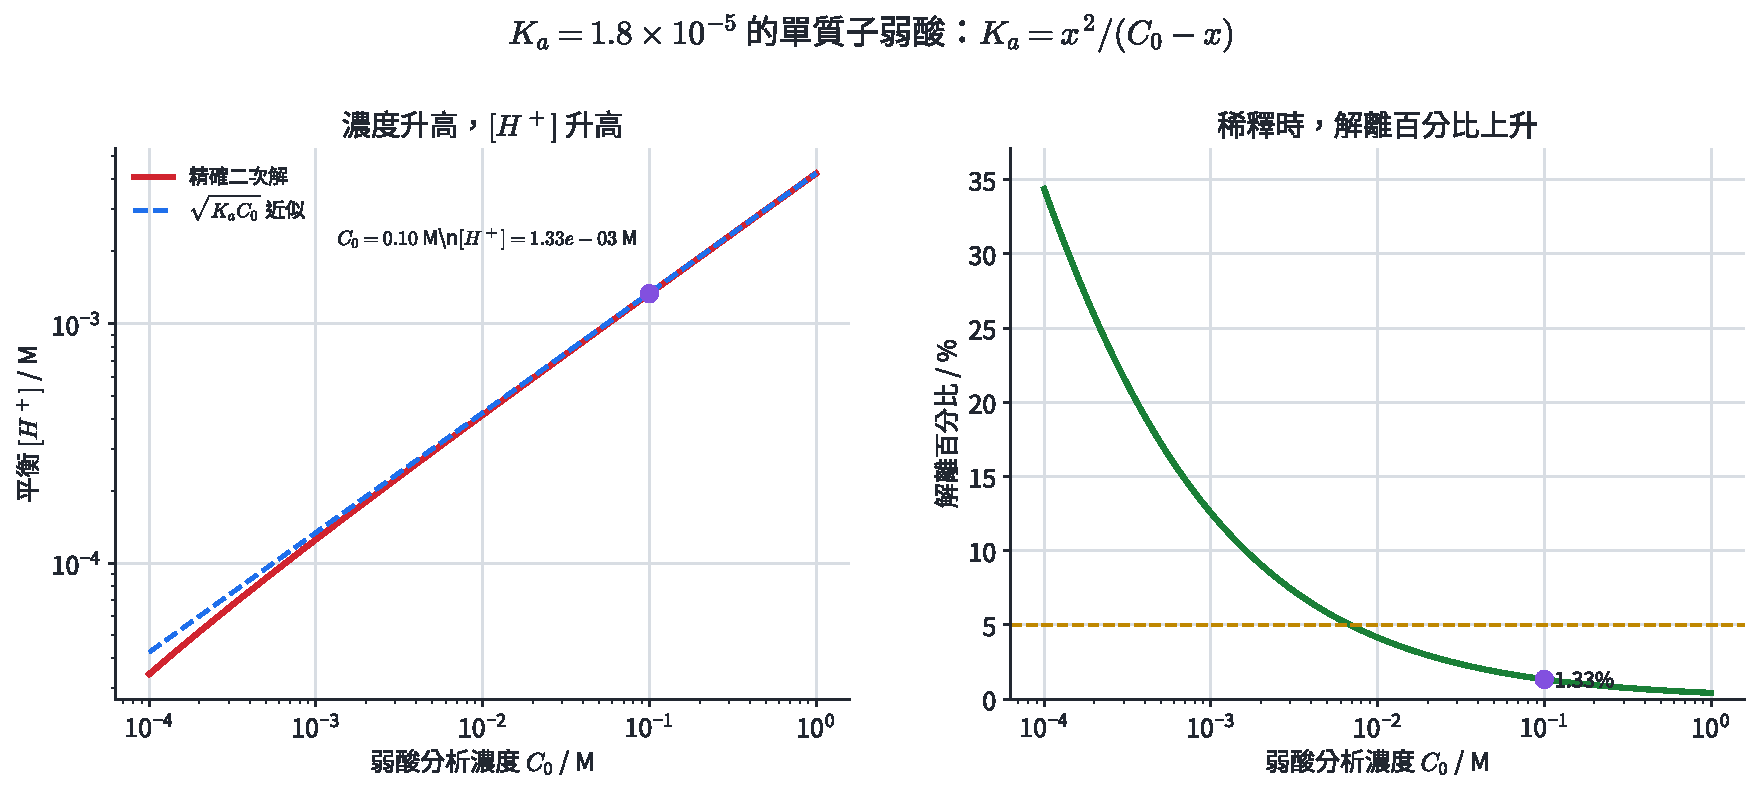
\includegraphics[width=0.97\linewidth,height=\textheight,keepaspectratio,alt={圖 4｜左圖比較精確二次解與平方根近似；右圖顯示稀釋時解離百分比上升。紫點是 0.10 M 醋酸的同一組數據。}]{assets/選化III-2-弱酸解離濃度與百分比.pdf}
\caption{圖 4｜左圖比較精確二次解與平方根近似；右圖顯示稀釋時解離百分比上升。紫點是 0.10 M 醋酸的同一組數據。}
\end{figure}

\subsection{4.2 平方根近似的檢查}\label{ux5e73ux65b9ux6839ux8fd1ux4f3cux7684ux6aa2ux67e5}

若計算後 \(x/C_0<5\%\)，可用 \(C_0-x\approx C_0\)：

\[
[H^+]\approx\sqrt{K_aC_0}.
\]

這是由完整平衡式得到的近似。計算順序是先求近似值，再以 \(x/C_0\) 檢查；比例過大時改解二次式。

\begin{HandoutWorkedExample}

\subsection{\texorpdfstring{示範 7｜由 \(K_a\) 求甲酸的 pH 與解離百分比}{示範 7｜由 K\_a 求甲酸的 pH 與解離百分比}}\label{ux793aux7bc4-7ux7531-k_a-ux6c42ux7532ux9178ux7684-ph-ux8207ux89e3ux96e2ux767eux5206ux6bd4}

\(25\,^\circ\mathrm C\) 時，\(0.100\ \mathrm M\) 甲酸的 \(K_a=1.8\times10^{-4}\)。完整方程為

\[
\frac{x^2}{0.100-x}=1.8\times10^{-4}.
\]

整理：

\[
x^2+(1.8\times10^{-4})x-1.8\times10^{-5}=0.
\]

正根為

\[
x=4.15\times10^{-3}\ \mathrm M.
\]

\[
pH=-\log(4.15\times10^{-3})=2.38,
\]

\[
\alpha=\frac{4.15\times10^{-3}}{0.100}\times100\%=4.15\%.
\]

解離比例低於 \(5\%\)，平方根估算 \(\sqrt{(1.8\times10^{-4})(0.100)}=4.24\times10^{-3}\) 與精確值接近。

\end{HandoutWorkedExample}

\begin{HandoutWorkedExample}

\subsection{\texorpdfstring{示範 8｜由 pH 反求未知弱酸的 \(K_a\)}{示範 8｜由 pH 反求未知弱酸的 K\_a}}\label{ux793aux7bc4-8ux7531-ph-ux53cdux6c42ux672aux77e5ux5f31ux9178ux7684-k_a}

\(0.0500\ \mathrm M\) 單質子弱酸的 pH 為 \(2.70\)。

\[
x=[H^+]=10^{-2.70}=2.00\times10^{-3}\ \mathrm M.
\]

平衡時 \([A^-]=x\)、\([HA]=0.0500-x=0.0480\ \mathrm M\)：

\[
K_a=\frac{x^2}{0.0500-x}
=\frac{(2.00\times10^{-3})^2}{0.0480}
=8.3\times10^{-5}.
\]

\[
\alpha=\frac{2.00\times10^{-3}}{0.0500}\times100\%=4.00\%.
\]

量得的 pH 與已知分析濃度共同決定平衡常數。

\end{HandoutWorkedExample}

弱酸平衡可連結食品酸度、藥物離子化、保存劑分布與水體酸化。\(K_a\) 描述平衡傾向；總酸量與滴定可中和的莫耳數還需由分析濃度和體積決定。

\subsection{分節練習 4}\label{ux5206ux7bc0ux7df4ux7fd2-4}

\begin{enumerate}
\def\labelenumi{\arabic{enumi}.}
\tightlist
\item
  \(0.200\ \mathrm M\) 醋酸的 \(K_a=1.8\times10^{-5}\)。求 \([H^+]\)、pH 與解離百分比。
\item
  同一醋酸稀釋成 \(0.0200\ \mathrm M\)。求 \([H^+]\) 與解離百分比，並與第 1 題比較。
\item
  \(0.100\ \mathrm M\) 單質子弱酸的 pH 為 \(3.00\)。求 \(K_a\) 與解離百分比。
\item
  \(C_0=4.0\times10^{-4}\ \mathrm M\)、\(K_a=1.0\times10^{-5}\)。檢查平方根近似是否適用，並求精確 \([H^+]\)。
\end{enumerate}

\subsection{分節練習 4 解析}\label{ux5206ux7bc0ux7df4ux7fd2-4-ux89e3ux6790}

\begin{enumerate}
\def\labelenumi{\arabic{enumi}.}
\tightlist
\item
  解
  \[
  \frac{x^2}{0.200-x}=1.8\times10^{-5}
  \]
  得 \(x=1.89\times10^{-3}\ \mathrm M\)。因此
  \[
  pH=2.72,\qquad
  \alpha=\frac{1.89\times10^{-3}}{0.200}\times100\%=0.944\%.
  \]
\item
  解
  \[
  \frac{x^2}{0.0200-x}=1.8\times10^{-5}
  \]
  得 \(x=5.91\times10^{-4}\ \mathrm M\)，pH \(=3.23\)，
  \[
  \alpha=\frac{5.91\times10^{-4}}{0.0200}\times100\%=2.96\%.
  \]
  稀釋後 \([H^+]\) 下降，而解離百分比上升。
\item
  \(x=10^{-3.00}=1.00\times10^{-3}\ \mathrm M\)：
  \[
  K_a=\frac{(1.00\times10^{-3})^2}{0.100-0.001}
  =1.01\times10^{-5}.
  \]
  \(\alpha=(0.001/0.100)\times100\%=1.00\%\)。
\item
  平方根估算為
  \[
  x\approx\sqrt{(1.0\times10^{-5})(4.0\times10^{-4})}
  =6.32\times10^{-5}\ \mathrm M,
  \]
  占 \(C_0\) 的 \(15.8\%\)，需解二次式：
  \[
  x^2+(1.0\times10^{-5})x-4.0\times10^{-9}=0.
  \]
  正根 \(x=5.84\times10^{-5}\ \mathrm M\)。
\end{enumerate}

\section{\texorpdfstring{5. 弱鹼的 \(K_b\) 與共軛常數}{5. 弱鹼的 K\_b 與共軛常數}}\label{ux5f31ux9e7cux7684-k_b-ux8207ux5171ux8edbux5e38ux6578}

\subsection{5.1 弱鹼解離與 pOH}\label{ux5f31ux9e7cux89e3ux96e2ux8207-poh}

以一元弱鹼 \(B\) 為例：

\[
B(aq)+H_2O(l)\rightleftharpoons BH^+(aq)+OH^-(aq),
\]

\[
K_b=\frac{[BH^+][OH^-]}{[B]}.
\]

初濃度為 \(C_0\) 且解離量為 \(x\) 時，

\[
K_b=\frac{x^2}{C_0-x},\qquad [OH^-]=x.
\]

求得 \([OH^-]\) 後先算 pOH，再用指定溫度的 \(pK_w\) 求 pH。

\subsection{\texorpdfstring{5.2 共軛酸鹼的 \(K_aK_b=K_w\)}{5.2 共軛酸鹼的 K\_aK\_b=K\_w}}\label{ux5171ux8edbux9178ux9e7cux7684-k_ak_bk_w}

對共軛對 \(HA/A^-\)：

\[
HA\rightleftharpoons H^++A^-,
\qquad
A^-+H_2O\rightleftharpoons HA+OH^-.
\]

相乘並約去 \(HA\)、\(A^-\) 後得到水的自解離：

\[
K_a(HA)K_b(A^-)=K_w.
\]

在 \(25\,^\circ\mathrm C\)，

\[
pK_a+pK_b=14.00.
\]

\begin{figure}
\centering
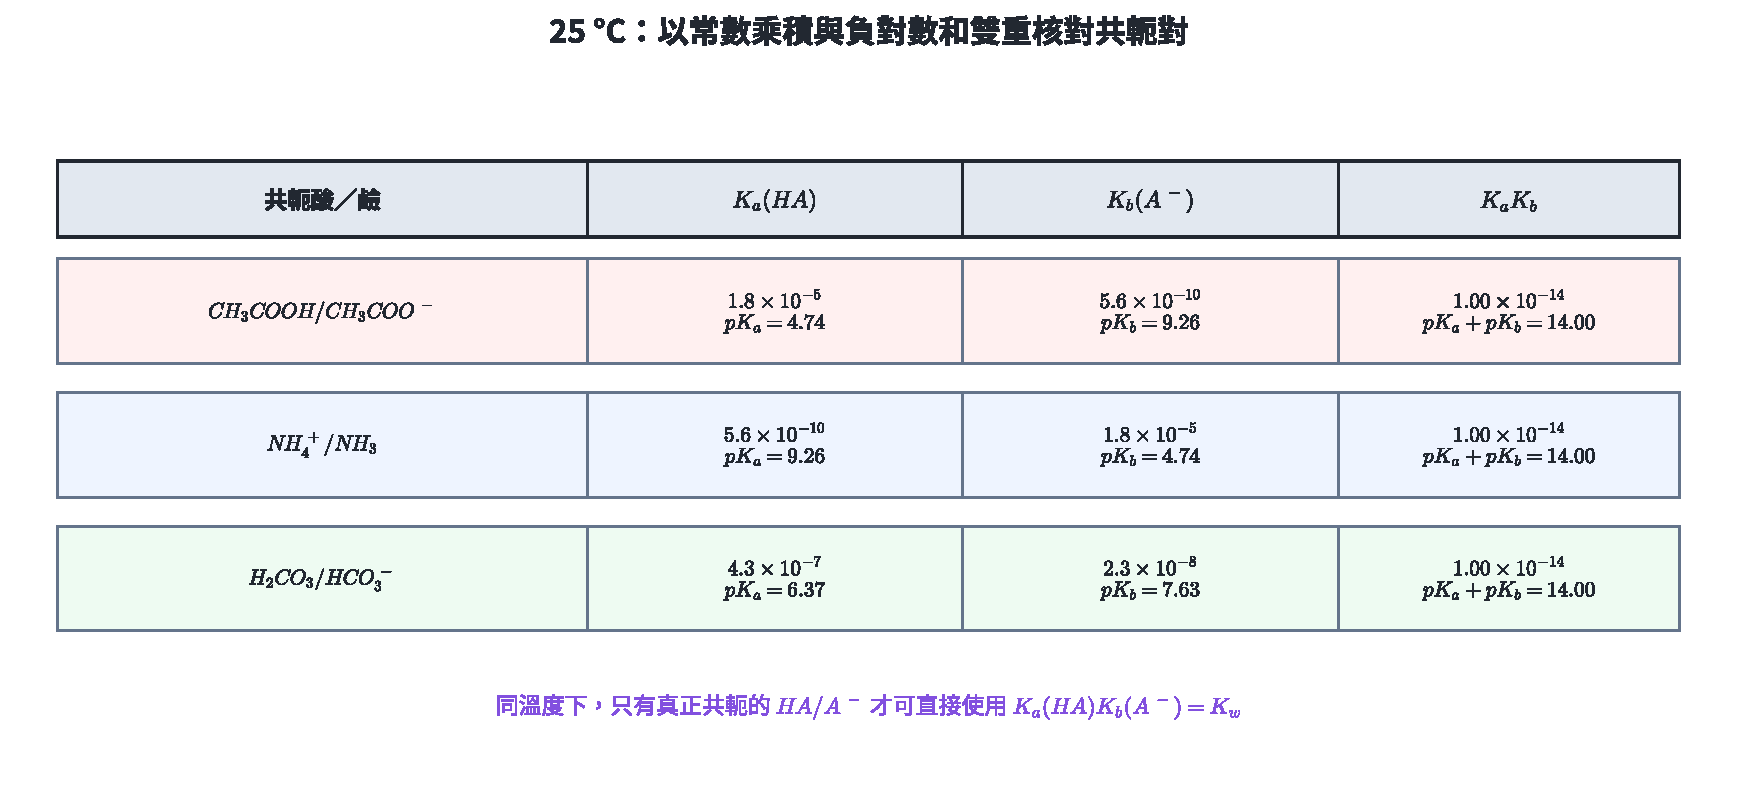
\includegraphics[width=0.94\linewidth,height=\textheight,keepaspectratio,alt={圖 5｜每一列是一組真正共軛的 HA/A\^{}-；向右依序核對 K\_a、K\_b、乘積 K\_w，並以 pK\_a+pK\_b=14.00 再檢查一次。}]{assets/選化III-2-共軛酸鹼KaKb.pdf}
\caption{圖 5｜每一列是一組真正共軛的 \(HA/A^-\)；向右依序核對 \(K_a\)、\(K_b\)、乘積 \(K_w\)，並以 \(pK_a+pK_b=14.00\) 再檢查一次。}
\end{figure}

酸愈強，其共軛鹼愈弱；鹼愈強，其共軛酸愈弱。這是同一個乘積固定關係的兩種說法。

\begin{HandoutWorkedExample}

\subsection{\texorpdfstring{示範 9｜由 \(K_b\) 求氨水的 pH}{示範 9｜由 K\_b 求氨水的 pH}}\label{ux793aux7bc4-9ux7531-k_b-ux6c42ux6c28ux6c34ux7684-ph}

\(25\,^\circ\mathrm C\) 時，\(0.100\ \mathrm M\) \(NH_3\) 的 \(K_b=1.8\times10^{-5}\)：

\[
NH_3+H_2O\rightleftharpoons NH_4^++OH^-.
\]

\[
\frac{x^2}{0.100-x}=1.8\times10^{-5}.
\]

正根為 \(x=1.33\times10^{-3}\ \mathrm M\)，所以

\[
pOH=2.875,\qquad pH=14.000-2.875=11.125.
\]

\[
\alpha=\frac{1.33\times10^{-3}}{0.100}\times100\%=1.33\%.
\]

\end{HandoutWorkedExample}

\begin{HandoutWorkedExample}

\subsection{示範 10｜由弱酸常數求共軛鹼常數}\label{ux793aux7bc4-10ux7531ux5f31ux9178ux5e38ux6578ux6c42ux5171ux8edbux9e7cux5e38ux6578}

醋酸的 \(K_a=1.8\times10^{-5}\)。醋酸根的 \(K_b\) 為

\[
K_b(CH_3COO^-)=\frac{K_w}{K_a}
=\frac{1.0\times10^{-14}}{1.8\times10^{-5}}
=5.56\times10^{-10}.
\]

醋酸是弱酸，醋酸根也是弱鹼；兩者的常數相差很大，顯示醋酸根接受水中質子的傾向很小。這個 \(K_b\) 會在醋酸鈉水解與弱酸滴定當量點再次使用。

\end{HandoutWorkedExample}

胺類的鹼性影響氣味控制、藥物鹽型與生物分子的帶電狀態。弱鹼計算描述指定溶液中的平衡濃度；揮發、離子強度與多個鹼性位置會使真實系統需要更多物種平衡。

\subsection{分節練習 5}\label{ux5206ux7bc0ux7df4ux7fd2-5}

\begin{enumerate}
\def\labelenumi{\arabic{enumi}.}
\tightlist
\item
  \(25\,^\circ\mathrm C\) 時，\(1.00\ \mathrm M\) 三甲胺 \((CH_3)_3N\) 的 \(K_b=6.4\times10^{-5}\)。求 \([OH^-]\)、pH 與解離百分比。
\item
  \(NH_3\) 的 \(K_b=1.8\times10^{-5}\)。求 \(NH_4^+\) 的 \(K_a\) 與 \(pK_a\)。
\item
  某弱酸 \(HA\) 的 \(K_a=4.0\times10^{-4}\)。求 \(A^-\) 的 \(K_b\)。
\item
  已知 \(K_a(HF)=7.2\times10^{-4}\)、\(K_a(HClO)=3.5\times10^{-8}\)。比較 \(F^-\)、\(ClO^-\) 的鹼性。
\end{enumerate}

\subsection{分節練習 5 解析}\label{ux5206ux7bc0ux7df4ux7fd2-5-ux89e3ux6790}

\begin{enumerate}
\def\labelenumi{\arabic{enumi}.}
\tightlist
\item
  解
  \[
  \frac{x^2}{1.00-x}=6.4\times10^{-5}
  \]
  得 \(x=7.97\times10^{-3}\ \mathrm M\)。因此
  \[
  pOH=2.099,\qquad pH=11.901,
  \]
  \[
  \alpha=\frac{7.97\times10^{-3}}{1.00}\times100\%=0.797\%.
  \]
\item
  \[
   K_a(NH_4^+)=\frac{10^{-14}}{1.8\times10^{-5}}
   =5.56\times10^{-10},
   \]
  \[
   pK_a=9.26.
   \]
\item
  \[
   K_b(A^-)=\frac{10^{-14}}{4.0\times10^{-4}}
   =2.5\times10^{-11}.
   \]
\item
  \(HClO\) 的 \(K_a\) 較小，是較弱的酸，因此其共軛鹼 \(ClO^-\) 較強。數值上
  \[
  K_b(F^-)=1.39\times10^{-11},\qquad
  K_b(ClO^-)=2.86\times10^{-7}.
  \]
\end{enumerate}

\section{6. 同離子效應}\label{ux540cux96e2ux5b50ux6548ux61c9}

\subsection{6.1 共同離子改變平衡組成}\label{ux5171ux540cux96e2ux5b50ux6539ux8b8aux5e73ux8861ux7d44ux6210}

弱酸平衡

\[
HA\rightleftharpoons H^++A^-
\]

若加入可溶性鹽 \(NaA\)，鹽完全解離提供 \(A^-\)。反應商

\[
Q_a=\frac{[H^+][A^-]}{[HA]}
\]

立即增大，系統向生成 \(HA\) 的方向調整，弱酸解離百分比降低。若初始已有 \([A^-]_0\)，令弱酸再解離 \(x\)：

\[
K_a=\frac{x([A^-]_0+x)}{[HA]_0-x}.
\]

當 \(x\) 相對於兩個初濃度都小，

\[
[H^+]\approx K_a\frac{[HA]_0}{[A^-]_0}.
\]

\begin{figure}
\centering
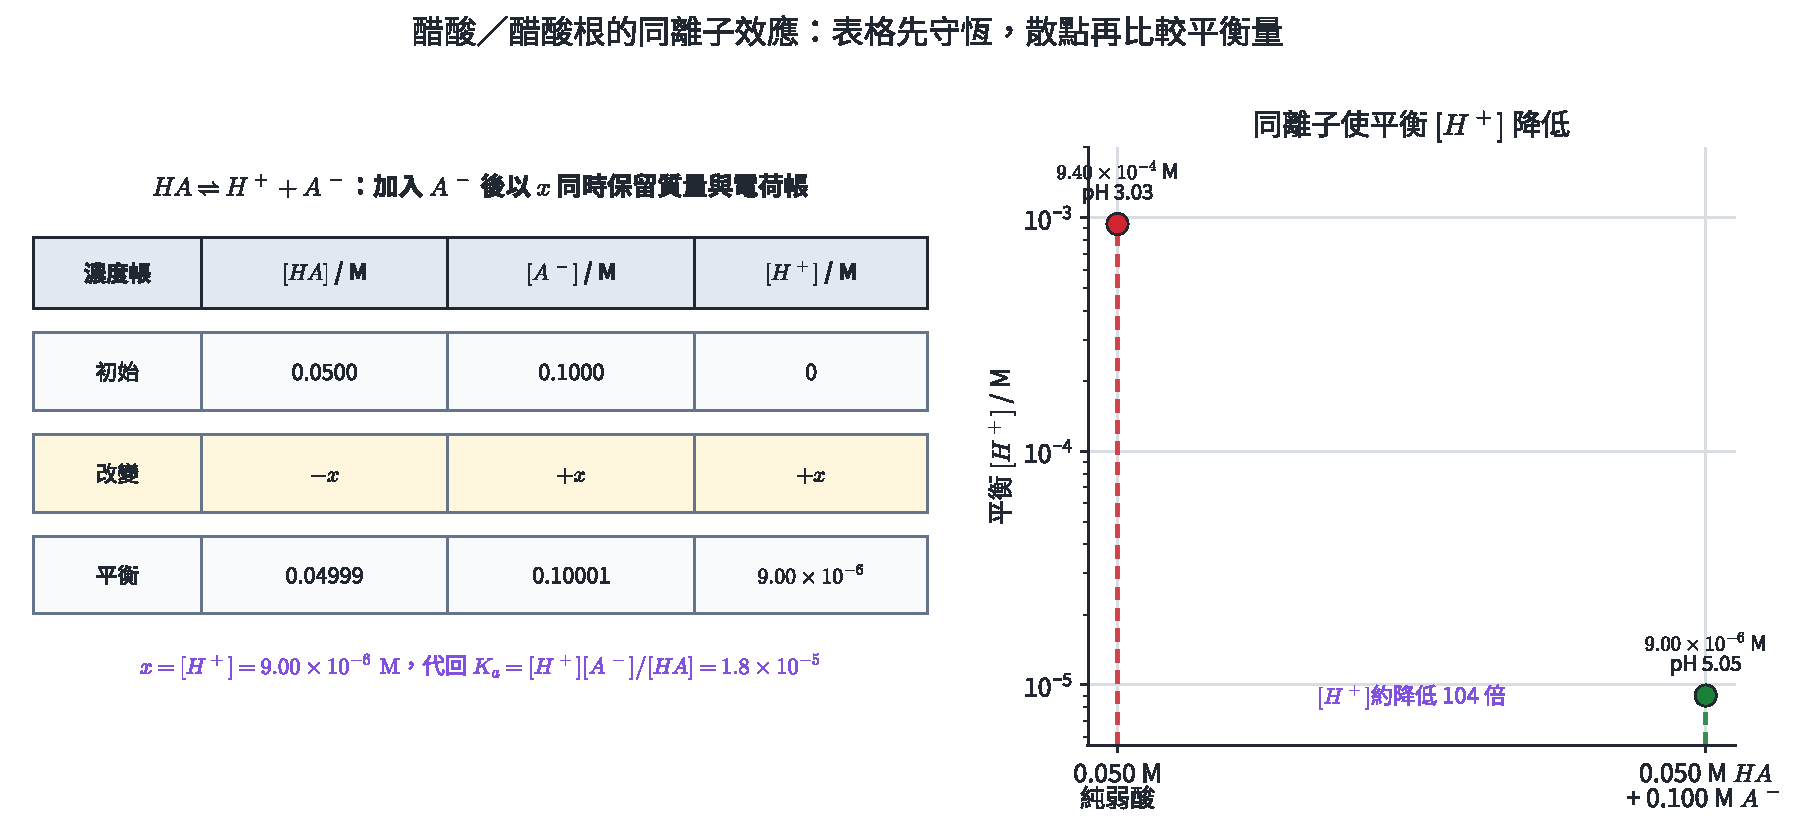
\includegraphics[width=0.97\linewidth,height=\textheight,keepaspectratio,alt={圖 6｜左圖以初始、改變、平衡帳同時追蹤 HA、A−與 H+；右圖的對數刻度顯示，加入 0.100 M A− 後，平衡氫離子濃度約降低 104 倍。}]{assets/選化III-2-同離子效應濃度帳.pdf}
\caption{圖 6｜左圖以初始、改變、平衡帳同時追蹤 HA、A−與 H+；右圖的對數刻度顯示，加入 0.100 M A− 後，平衡氫離子濃度約降低 104 倍。}
\end{figure}

\subsection{6.2 強酸或強鹼提供的同離子}\label{ux5f37ux9178ux6216ux5f37ux9e7cux63d0ux4f9bux7684ux540cux96e2ux5b50}

在弱酸溶液加入強酸，外加的 \(H^+\) 抑制弱酸解離；在弱鹼溶液加入強鹼，外加的 \(OH^-\) 抑制弱鹼解離。計算時先確認強電解質的初始濃度，再寫弱電解質的微小平衡改變。

\begin{HandoutWorkedExample}

\subsection{示範 11｜醋酸與醋酸鈉混合}\label{ux793aux7bc4-11ux918bux9178ux8207ux918bux9178ux9209ux6df7ux5408}

等體積混合 \(0.100\ \mathrm M\) \(CH_3COOH\) 與 \(0.200\ \mathrm M\) \(CH_3COONa\)。混合後

\[
[CH_3COOH]_0=0.0500\ \mathrm M,\qquad
[CH_3COO^-]_0=0.100\ \mathrm M.
\]

\(K_a=1.8\times10^{-5}\)：

\[
1.8\times10^{-5}
=\frac{x(0.100+x)}{0.0500-x}.
\]

精確解為

\[
[H^+]=x=9.00\times10^{-6}\ \mathrm M,
\qquad pH=5.046.
\]

醋酸解離百分比為

\[
\alpha=\frac{9.00\times10^{-6}}{0.0500}\times100\%
=0.0180\%.
\]

相同濃度的純醋酸會有更高的 \([H^+]\)；差異來自初始醋酸根改變了反應商。

\end{HandoutWorkedExample}

\begin{HandoutWorkedExample}

\subsection{示範 12｜強鹼抑制氨的解離}\label{ux793aux7bc4-12ux5f37ux9e7cux6291ux5236ux6c28ux7684ux89e3ux96e2}

某溫度下 \(K_b(NH_3)=1.0\times10^{-5}\)。在 \(0.100\ \mathrm M\) \(NH_3\) 中加入 \(NaOH\)，使初始 \([OH^-]=0.100\ \mathrm M\)。令氨再反應 \(x\)：

\[
K_b=\frac{x(0.100+x)}{0.100-x}.
\]

\(x\) 很小，可先估算

\[
x\approx K_b\frac{[NH_3]}{[OH^-]}
=(1.0\times10^{-5})\frac{0.100}{0.100}
=1.0\times10^{-5}\ \mathrm M.
\]

氨的解離百分比約為

\[
\frac{1.0\times10^{-5}}{0.100}\times100\%=0.010\%.
\]

純 \(0.100\ \mathrm M\) 氨水約有 \(1.0\%\) 解離；共同 \(OH^-\) 使解離比例約降為原來的百分之一。

\end{HandoutWorkedExample}

同離子效應是緩衝液、藥物鹽析、沉澱控制與分析化學分離的共同機制。它改變的是平衡組成；若加入物同時與原物種發生定量中和，需先完成化學計量，再建立新的平衡。

\subsection{分節練習 6}\label{ux5206ux7bc0ux7df4ux7fd2-6}

\begin{enumerate}
\def\labelenumi{\arabic{enumi}.}
\tightlist
\item
  \(0.100\ \mathrm M\) 弱酸 \(HA\)（\(K_a=2.0\times10^{-5}\)）同時含 \(0.0100\ \mathrm M\) \(HCl\)。求平衡 \([A^-]\) 與 \(HA\) 的解離百分比。
\item
  等體積混合 \(0.200\ \mathrm M\) \(NH_3\) 與 \(0.100\ \mathrm M\) \(NH_4Cl\)。已知 \(K_b=1.8\times10^{-5}\)，求 pH。
\item
  \(0.0500\ \mathrm M\) 醋酸在純水中的解離百分比約為多少？若同時含 \(0.100\ \mathrm M\) 醋酸根，解離百分比約為多少？
\item
  三杯溶液均含 \(0.100\ \mathrm M\) 醋酸：甲為純醋酸；乙另含 \(0.0500\ \mathrm M\) \(HCl\)；丙另含 \(0.0500\ \mathrm M\) \(CH_3COONa\)。依醋酸解離百分比由大到小排列。
\end{enumerate}

\subsection{分節練習 6 解析}\label{ux5206ux7bc0ux7df4ux7fd2-6-ux89e3ux6790}

\begin{enumerate}
\def\labelenumi{\arabic{enumi}.}
\tightlist
\item
  令 \(HA\) 解離 \(x\)：
  \[
  2.0\times10^{-5}
  =\frac{x(0.0100+x)}{0.100-x}.
  \]
  正根 \(x=1.96\times10^{-4}\ \mathrm M\)，所以
  \[
  [A^-]=1.96\times10^{-4}\ \mathrm M,
  \qquad
  \alpha=0.196\%.
  \]
\item
  混合後 \([NH_3]_0=0.100\ \mathrm M\)、\([NH_4^+]_0=0.0500\ \mathrm M\)：
  \[
  [OH^-]\approx K_b\frac{[NH_3]}{[NH_4^+]}
  =(1.8\times10^{-5})\frac{0.100}{0.0500}
  =3.6\times10^{-5}\ \mathrm M.
  \]
  \(pOH=4.44\)，所以 \(pH=9.56\)。
\item
  純醋酸：
  \[
  [H^+]\approx\sqrt{(1.8\times10^{-5})(0.0500)}
  =9.49\times10^{-4}\ \mathrm M,
  \]
  \(\alpha\approx1.90\%\)。加入 \(0.100\ \mathrm M\) 醋酸根後，
  \[
  [H^+]\approx(1.8\times10^{-5})\frac{0.0500}{0.100}
  =9.0\times10^{-6}\ \mathrm M,
  \]
  \(\alpha\approx0.0180\%\)。
\item
  甲沒有外加同離子，解離比例最大。乙與丙的平衡變化量都可記為 \(x\)，且都滿足
  \[
  K_a=\frac{x(0.0500+x)}{0.100-x}.
  \]
  解得 \(x=3.60\times10^{-5}\ \mathrm M\)，解離百分率都是 \(0.0360\%\)。因此排列為甲 \(>\) 乙 \(=\) 丙。
\end{enumerate}

\section{7. 多質子酸、質量平衡與物種分布}\label{ux591aux8ceaux5b50ux9178ux8ceaux91cfux5e73ux8861ux8207ux7269ux7a2eux5206ux5e03}

\subsection{7.1 逐步解離常數}\label{ux9010ux6b65ux89e3ux96e2ux5e38ux6578}

二質子酸 \(H_2A\) 分兩步解離：

\[
H_2A\rightleftharpoons H^++HA^-,
\qquad
K_{a1}=\frac{[H^+][HA^-]}{[H_2A]},
\]

\[
HA^-\rightleftharpoons H^++A^{2-},
\qquad
K_{a2}=\frac{[H^+][A^{2-}]}{[HA^-]}.
\]

一般有 \(K_{a1}>K_{a2}\)，因為從帶負電的粒子再移走正電質子需要更高能量。當兩個常數相差數個數量級，初始酸溶液的 \([H^+]\) 主要由第一步決定；第二步則決定少量高電荷酸根的濃度。

\subsection{7.2 質量平衡與電荷平衡}\label{ux8ceaux91cfux5e73ux8861ux8207ux96fbux8377ux5e73ux8861}

分析濃度 \(C_0\) 的二質子酸滿足

\[
C_0=[H_2A]+[HA^-]+[A^{2-}].
\]

若溶液中沒有其他離子，

\[
[H^+]=[OH^-]+[HA^-]+2[A^{2-}].
\]

前式追蹤所有含 \(A\) 的物種，後式追蹤正、負電荷。多個平衡式需配合這兩條守恆關係，才能決定全部濃度。

\subsection{7.3 pH 決定主要物種}\label{ph-ux6c7aux5b9aux4e3bux8981ux7269ux7a2e}

對二質子酸，物種分率為

\[
\alpha_{H_2A}=\frac{[H^+]^2}{D},\qquad
\alpha_{HA^-}=\frac{K_{a1}[H^+]}{D},\qquad
\alpha_{A^{2-}}=\frac{K_{a1}K_{a2}}{D},
\]

\[
D=[H^+]^2+K_{a1}[H^+]+K_{a1}K_{a2}.
\]

三個分率相加為 \(1\)。在 \(pH=pK_{a1}\) 時 \([H_2A]=[HA^-]\)；在 \(pH=pK_{a2}\) 時 \([HA^-]=[A^{2-}]\)。

\begin{figure}
\centering
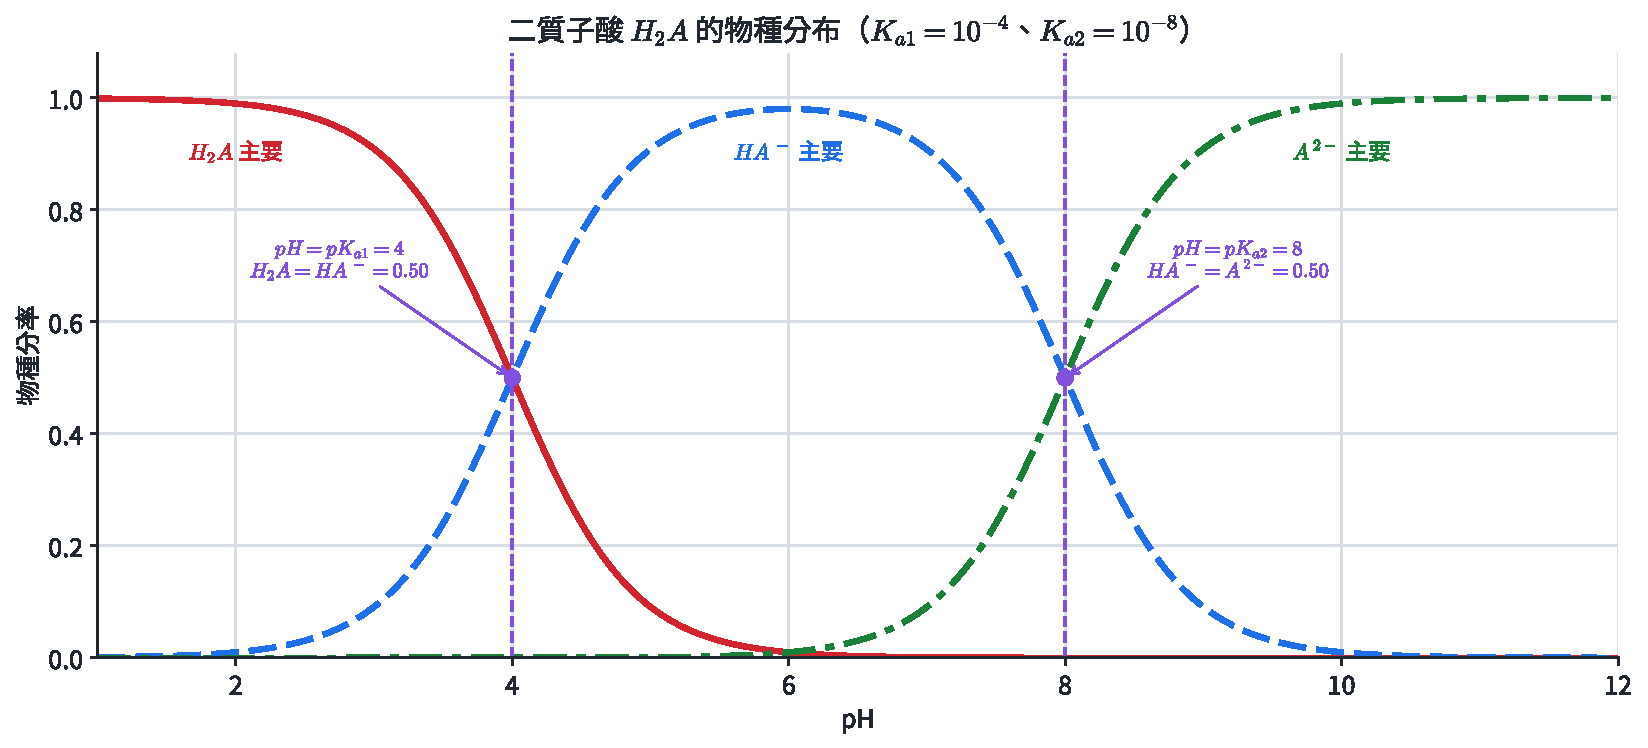
\includegraphics[width=0.95\linewidth,height=\textheight,keepaspectratio,alt={圖 7｜實線、虛線與點鏈線分別表示 H2A、HA− 與 A2−；pH = pKa1 及 pKa2 的交點都對應相鄰物種各占 0.50。}]{assets/選化III-2-二質子酸物種分布.pdf}
\caption{圖 7｜實線、虛線與點鏈線分別表示 H2A、HA− 與 A2−；pH = pKa1 及 pKa2 的交點都對應相鄰物種各占 0.50。}
\end{figure}

\begin{HandoutWorkedExample}

\subsection{\texorpdfstring{示範 13｜\(H_2S\) 的兩步解離}{示範 13｜H\_2S 的兩步解離}}\label{ux793aux7bc4-13h_2s-ux7684ux5169ux6b65ux89e3ux96e2}

\(0.100\ \mathrm M\) \(H_2S\) 有 \(K_{a1}=1.0\times10^{-7}\)、\(K_{a2}=1.2\times10^{-14}\)。第一步近似：

\[
[H^+]\approx\sqrt{K_{a1}C_0}
=\sqrt{(1.0\times10^{-7})(0.100)}
=1.0\times10^{-4}\ \mathrm M,
\]

所以 pH 約為 \(4.00\)，且 \([HS^-]\approx1.0\times10^{-4}\ \mathrm M\)。

第二步：

\[
K_{a2}=\frac{[H^+][S^{2-}]}{[HS^-]}.
\]

因 \([H^+]\approx[HS^-]\)，

\[
[S^{2-}]\approx K_{a2}=1.2\times10^{-14}\ \mathrm M.
\]

兩個 \(K_a\) 相差近七個數量級，因此第二步對總 \([H^+]\) 的貢獻極小。

\end{HandoutWorkedExample}

\begin{HandoutWorkedExample}

\subsection{\texorpdfstring{示範 14｜兩性離子 \(HCO_3^-\) 的近似 pH}{示範 14｜兩性離子 HCO\_3\^{}- 的近似 pH}}\label{ux793aux7bc4-14ux5169ux6027ux96e2ux5b50-hco_3--ux7684ux8fd1ux4f3c-ph}

\(HCO_3^-\) 可向下解離，也可向上接受質子。對主要由單一兩性物種形成的稀溶液，

\[
pH\approx\frac12(pK_{a1}+pK_{a2}).
\]

碳酸的 \(K_{a1}=4.3\times10^{-7}\)、\(K_{a2}=5.6\times10^{-11}\)：

\[
pK_{a1}=6.37,\qquad pK_{a2}=10.25,
\]

\[
pH\approx\frac{6.37+10.25}{2}=8.31.
\]

\(HCO_3^-\) 的接受質子傾向在此條件下稍強於提供質子的傾向，所以碳酸氫鈉水溶液呈弱鹼性。

\end{HandoutWorkedExample}

多質子酸分布可用於磷酸鹽緩衝、天然水碳酸系、胺基酸帶電狀態與分段滴定。物種分布圖使用平衡常數與 pH；若同時含金屬配位或沉澱，還需加入相應平衡。

\subsection{分節練習 7}\label{ux5206ux7bc0ux7df4ux7fd2-7}

\begin{enumerate}
\def\labelenumi{\arabic{enumi}.}
\tightlist
\item
  寫出 \(H_3PO_4\) 的三步解離反應與 \(K_{a1}\)、\(K_{a2}\)、\(K_{a3}\) 表示式。
\item
  對分析濃度為 \(C_0\) 的 \(H_3PO_4\) 水溶液，寫出磷酸物種的質量平衡與溶液電荷平衡。
\item
  同濃度順丁烯二酸與反丁烯二酸的 \(K_{a1}\) 分別為 \(1.2\times10^{-2}\)、\(1.0\times10^{-3}\)。哪一杯初始 \([H^+]\) 較大？
\item
  某二質子酸有 \(pK_{a1}=4.0\)、\(pK_{a2}=8.0\)。判斷 pH \(=2.0\)、\(6.0\)、\(10.0\) 時的主要物種。
\end{enumerate}

\subsection{分節練習 7 解析}\label{ux5206ux7bc0ux7df4ux7fd2-7-ux89e3ux6790}

\begin{enumerate}
\def\labelenumi{\arabic{enumi}.}
\tightlist
\item
  \[
   H_3PO_4\rightleftharpoons H^++H_2PO_4^-,
   \qquad
   K_{a1}=\frac{[H^+][H_2PO_4^-]}{[H_3PO_4]},
   \]
  \[
   H_2PO_4^-\rightleftharpoons H^++HPO_4^{2-},
   \qquad
   K_{a2}=\frac{[H^+][HPO_4^{2-}]}{[H_2PO_4^-]},
   \]
  \[
   HPO_4^{2-}\rightleftharpoons H^++PO_4^{3-},
   \qquad
   K_{a3}=\frac{[H^+][PO_4^{3-}]}{[HPO_4^{2-}]}.
   \]
\item
  質量平衡：
  \[
   C_0=[H_3PO_4]+[H_2PO_4^-]+[HPO_4^{2-}]+[PO_4^{3-}].
   \]
  電荷平衡：
  \[
   [H^+]=[OH^-]+[H_2PO_4^-]+2[HPO_4^{2-}]+3[PO_4^{3-}].
   \]
\item
  相同濃度下，\(K_{a1}\) 較大的順丁烯二酸第一步解離較多，因此初始 \([H^+]\) 較大。
\item
  pH \(2.0<pK_{a1}\)，主要為 \(H_2A\)；\(pK_{a1}<6.0<pK_{a2}\)，主要為 \(HA^-\)；pH \(10.0>pK_{a2}\)，主要為 \(A^{2-}\)。
\end{enumerate}

\section{8. 鹽的分類、命名與組成}\label{ux9e7dux7684ux5206ux985eux547dux540dux8207ux7d44ux6210}

\subsection{8.1 由取代程度分類}\label{ux7531ux53d6ux4ee3ux7a0bux5ea6ux5206ux985e}

鹽是由陽離子與陰離子組成的離子化合物，可由酸中可解離的 \(H^+\) 或鹼中可解離的 \(OH^-\) 被取代的程度分類：

\begin{itemize}
\tightlist
\item
  \textbf{正鹽：}可解離的 \(H^+\) 或 \(OH^-\) 全部被取代，例如 \(NaCl\)、\(Na_3PO_4\)、\(Na_2HPO_3\)。
\item
  \textbf{酸式鹽：}多質子酸仍保留至少一個可解離 \(H^+\)，例如 \(NaHCO_3\)、\(NaH_2PO_4\)。
\item
  \textbf{鹼式鹽：}多元鹼仍保留可解離 \(OH^-\)，例如 \(Ca(OH)Cl\)。
\item
  \textbf{複鹽：}晶體含兩種以上陽離子或陰離子，溶於水後解離成各簡單離子，例如 \(KAl(SO_4)_2\cdot12H_2O\)。
\item
  \textbf{錯鹽：}含錯離子；錯離子的結構與反應在選修化學 IV 再完整處理。
\end{itemize}

分類依可解離位置判定。\(NaH_2PO_2\) 中的兩個 \(P-H\) 不屬酸性質子，因此它是正鹽；\(NaH_2PO_3\) 仍保留一個 \(O-H\)，所以是酸式鹽。

\subsection{8.2 名稱由離子組成決定}\label{ux540dux7a31ux7531ux96e2ux5b50ux7d44ux6210ux6c7aux5b9a}

正鹽通常命名為「陰離子名＋陽離子名」。酸式鹽在酸根名稱中保留「氫」與數目，例如 \(NaH_2PO_4\) 為磷酸二氫鈉；鹼式鹽同時列出陰離子與氫氧根，例如 \(Cu(OH)Cl\) 為氯化氫氧銅（2）。

\begin{HandoutWorkedExample}

\subsection{示範 15｜命名與分類四種鹽}\label{ux793aux7bc4-15ux547dux540dux8207ux5206ux985eux56dbux7a2eux9e7d}

\begin{enumerate}
\def\labelenumi{\arabic{enumi}.}
\tightlist
\item
  \(NH_4Cl\)：氯化銨；可解離質子已全部被取代，是正鹽。
\item
  \(NH_4HC_2O_4\)：草酸氫銨；\(HC_2O_4^-\) 仍有可解離質子，是酸式鹽。
\item
  \(Ca(OH)Cl\)：氯化氫氧鈣；仍含可解離 \(OH^-\)，是鹼式鹽。
\item
  \(MgNH_4PO_4\)：磷酸銨鎂；含 \(Mg^{2+}\)、\(NH_4^+\) 兩種陽離子，是複鹽。
\end{enumerate}

分類只描述鹽的組成；水溶液的酸鹼性需再分析離子水解。

\end{HandoutWorkedExample}

\begin{HandoutWorkedExample}

\subsection{\texorpdfstring{示範 16｜比較 \(H_3PO_2\)、\(H_3PO_3\) 形成的鈉鹽}{示範 16｜比較 H\_3PO\_2、H\_3PO\_3 形成的鈉鹽}}\label{ux793aux7bc4-16ux6bd4ux8f03-h_3po_2h_3po_3-ux5f62ux6210ux7684ux9209ux9e7d}

\(H_3PO_2=H_2PO(OH)\) 是單質子酸，完全中和：

\[
H_3PO_2+NaOH\rightarrow NaH_2PO_2+H_2O.
\]

\(NaH_2PO_2\) 已無可解離 \(O-H\)，所以是正鹽。

\(H_3PO_3=HPO(OH)_2\) 是二質子酸，加入一當量 \(NaOH\)：

\[
H_3PO_3+NaOH\rightarrow NaH_2PO_3+H_2O.
\]

\(NaH_2PO_3\) 還有一個可解離 \(O-H\)，所以是酸式鹽。再加一當量 \(NaOH\) 得正鹽 \(Na_2HPO_3\)。

\end{HandoutWorkedExample}

鹽的組成連到肥料配方、食品膨鬆劑、凝聚劑與醫藥鹽型。名稱能指出離子來源；材料用途、毒性與溶解度仍需另外查驗物性與安全資料。

\subsection{分節練習 8}\label{ux5206ux7bc0ux7df4ux7fd2-8}

\begin{enumerate}
\def\labelenumi{\arabic{enumi}.}
\tightlist
\item
  命名並分類 \(NaHCO_3\)、\(Na_2HPO_4\)、\(Cu(OH)NO_3\)、\(KAl(SO_4)_2\cdot12H_2O\)。
\item
  判斷 \(NaH_2PO_2\)、\(NaH_2PO_3\)、\(Na_2HPO_3\) 中哪些是酸式鹽。
\item
  寫出由 \(H_2SO_3\) 依序與一當量、兩當量 \(NaOH\) 反應所得鹽的化學式與名稱。
\item
  某鹽溶於水得到 \(K^+\)、\(Al^{3+}\)、\(SO_4^{2-}\)，其最簡組成符合電荷守恆且同時含兩種陽離子。寫出無水鹽化學式並分類。
\end{enumerate}

\subsection{分節練習 8 解析}\label{ux5206ux7bc0ux7df4ux7fd2-8-ux89e3ux6790}

\begin{enumerate}
\def\labelenumi{\arabic{enumi}.}
\tightlist
\item
  \(NaHCO_3\)：碳酸氫鈉，酸式鹽；\(Na_2HPO_4\)：磷酸氫二鈉，酸式鹽；\(Cu(OH)NO_3\)：硝酸氫氧銅（2），鹼式鹽；\(KAl(SO_4)_2\cdot12H_2O\)：硫酸鋁鉀十二水合物，複鹽。
\item
  \(NaH_2PO_2\) 是正鹽；\(NaH_2PO_3\) 是酸式鹽；\(Na_2HPO_3\) 是正鹽。
\item
  一當量：
  \[
  H_2SO_3+NaOH\rightarrow NaHSO_3+H_2O,
  \]
  生成亞硫酸氫鈉。兩當量：
  \[
  H_2SO_3+2NaOH\rightarrow Na_2SO_3+2H_2O,
  \]
  生成亞硫酸鈉。
\item
  一個 \(K^+\) 與一個 \(Al^{3+}\) 共帶 \(+4\)，需兩個 \(SO_4^{2-}\) 平衡，所以化學式為 \(KAl(SO_4)_2\)，屬複鹽。
\end{enumerate}

\section{9. 鹽類水解與水溶液酸鹼性}\label{ux9e7dux985eux6c34ux89e3ux8207ux6c34ux6eb6ux6db2ux9178ux9e7cux6027}

\subsection{9.1 共軛離子與水反應}\label{ux5171ux8edbux96e2ux5b50ux8207ux6c34ux53cdux61c9}

鹽溶於水後先完全解離。弱酸的共軛鹼可由水取得質子：

\[
A^-+H_2O\rightleftharpoons HA+OH^-,
\]

\[
K_b(A^-)=\frac{K_w}{K_a(HA)}.
\]

弱鹼的共軛酸可把質子交給水：

\[
BH^++H_2O\rightleftharpoons B+H_3O^+,
\]

\[
K_a(BH^+)=\frac{K_w}{K_b(B)}.
\]

因此可依來源快速建立模型：

{\def\LTcaptype{none} % do not increment counter
\begin{longtable}[]{@{}lll@{}}
\toprule\noalign{}
鹽的來源 & 主要離子行為 & 水溶液傾向 \\
\midrule\noalign{}
\endhead
\bottomrule\noalign{}
\endlastfoot
強酸＋強鹼 & 兩離子與水的酸鹼反應極弱 & 中性 \\
弱酸＋強鹼 & 陰離子水解生成 \(OH^-\) & 鹼性 \\
強酸＋弱鹼 & 陽離子水解生成 \(H_3O^+\) & 酸性 \\
弱酸＋弱鹼 & 比較陰離子 \(K_b\) 與陽離子 \(K_a\) & 較大者主導 \\
\end{longtable}
}

鹽的「正鹽、酸式鹽、鹼式鹽」分類描述組成，水溶液酸鹼性描述水解平衡；兩者需分開判斷。

\begin{figure}
\centering
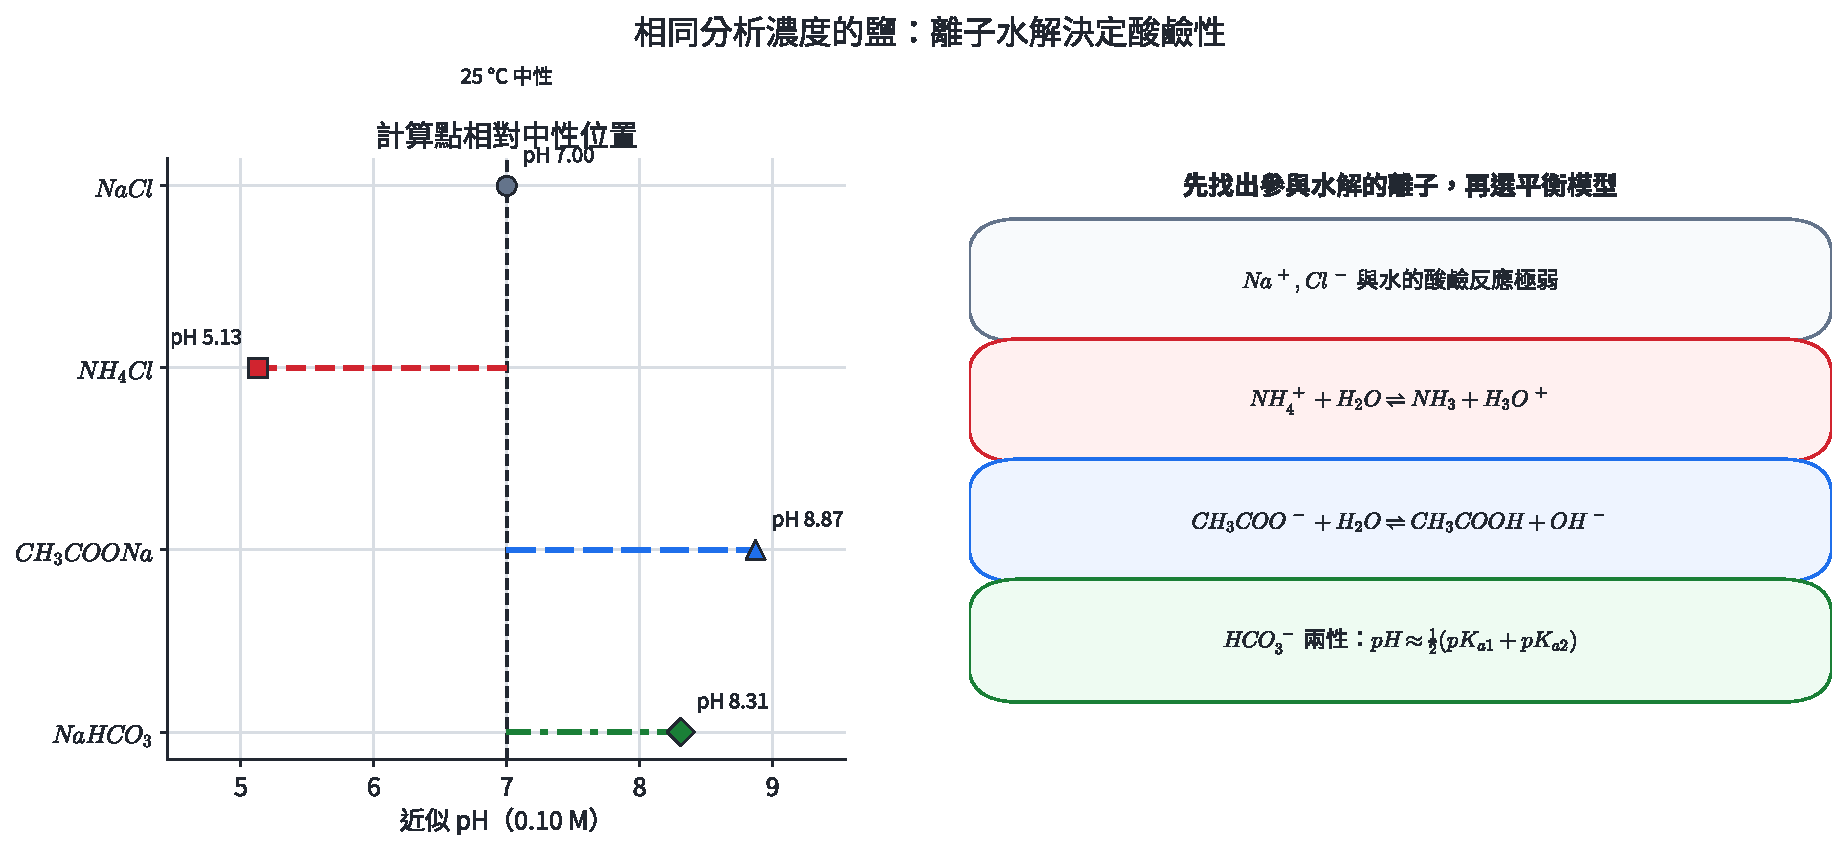
\includegraphics[width=0.95\linewidth,height=\textheight,keepaspectratio,alt={圖 8｜左圖以 25 °C 中性位置為基準標出四種 0.10 M 鹽的計算 pH；右圖列出各計算點對應的水解或兩性模型。}]{assets/選化III-2-鹽類水解與pH.pdf}
\caption{圖 8｜左圖以 25 °C 中性位置為基準標出四種 0.10 M 鹽的計算 pH；右圖列出各計算點對應的水解或兩性模型。}
\end{figure}

\subsection{9.2 兩性酸根的競爭}\label{ux5169ux6027ux9178ux6839ux7684ux7af6ux722d}

\(HA^-\) 這類兩性酸根可解離成 \(A^{2-}\)，也可水解成 \(H_2A\)。比較

\[
K_a(HA^-)=K_{a2},
\qquad
K_b(HA^-)=\frac{K_w}{K_{a1}}.
\]

\(K_a>K_b\) 時酸性反應較強；\(K_b>K_a\) 時鹼性反應較強。單一兩性物種主導且溶液不過度稀薄時，也可用

\[
pH\approx\frac12(pK_{a1}+pK_{a2})
\]

估算。

\begin{HandoutWorkedExample}

\subsection{示範 17｜醋酸鈉水解的 pH}\label{ux793aux7bc4-17ux918bux9178ux9209ux6c34ux89e3ux7684-ph}

\(25\,^\circ\mathrm C\) 時，\(0.100\ \mathrm M\) \(CH_3COONa\)，已知
\(K_a(CH_3COOH)=1.8\times10^{-5}\)。

\[
K_b(CH_3COO^-)=\frac{10^{-14}}{1.8\times10^{-5}}
=5.56\times10^{-10}.
\]

\[
CH_3COO^-+H_2O\rightleftharpoons CH_3COOH+OH^-.
\]

\[
\frac{x^2}{0.100-x}=5.56\times10^{-10}.
\]

解得 \([OH^-]=7.45\times10^{-6}\ \mathrm M\)，

\[
pOH=5.128,\qquad pH=8.872.
\]

\(Na^+\) 只負責電荷與總濃度，不提供主要酸鹼反應。

\end{HandoutWorkedExample}

\begin{HandoutWorkedExample}

\subsection{示範 18｜氯化銨水解的 pH}\label{ux793aux7bc4-18ux6c2fux5316ux92a8ux6c34ux89e3ux7684-ph}

\(0.0500\ \mathrm M\) \(NH_4Cl\)，\(K_b(NH_3)=1.8\times10^{-5}\)：

\[
K_a(NH_4^+)=\frac{10^{-14}}{1.8\times10^{-5}}
=5.56\times10^{-10}.
\]

\[
NH_4^++H_2O\rightleftharpoons NH_3+H_3O^+.
\]

\[
\frac{x^2}{0.0500-x}=5.56\times10^{-10}.
\]

解得 \([H^+]=5.27\times10^{-6}\ \mathrm M\)，所以

\[
pH=5.278.
\]

同一組 \(NH_4^+/NH_3\) 在弱鹼溶液、鹽類水解、緩衝液與滴定當量點中使用同一對常數。

\end{HandoutWorkedExample}

鹽類水解可解釋肥料、天然水、清潔鹽與藥物鹽的 pH。溶液實際 pH 還受濃度、溫度、二氧化碳吸收、沉澱與配位影響；題目給定額外反應時需一併列入物種帳。

\subsection{分節練習 9}\label{ux5206ux7bc0ux7df4ux7fd2-9}

\begin{enumerate}
\def\labelenumi{\arabic{enumi}.}
\tightlist
\item
  判斷 \(NaNO_3\)、\(NH_4Br\)、\(NaF\)、\(NH_4CN\) 水溶液的酸鹼模型；最後一種寫出需要比較的兩個常數。
\item
  求 \(25\,^\circ\mathrm C\)、\(0.200\ \mathrm M\) \(NaF\) 的 pH。已知 \(K_a(HF)=7.2\times10^{-4}\)。
\item
  判斷 \(NH_4F\) 水溶液偏酸或偏鹼。已知 \(K_b(NH_3)=1.8\times10^{-5}\)、\(K_a(HF)=7.2\times10^{-4}\)。
\item
  已知碳酸的 \(K_{a1}=4.3\times10^{-7}\)、\(K_{a2}=5.6\times10^{-11}\)。估算主要含 \(HCO_3^-\) 的碳酸氫鈉溶液 pH。
\end{enumerate}

\subsection{分節練習 9 解析}\label{ux5206ux7bc0ux7df4ux7fd2-9-ux89e3ux6790}

\begin{enumerate}
\def\labelenumi{\arabic{enumi}.}
\tightlist
\item
  \(NaNO_3\) 來自強酸、強鹼，模型為中性；\(NH_4Br\) 由 \(NH_4^+\) 水解，呈酸性；\(NaF\) 由 \(F^-\) 水解，呈鹼性。\(NH_4CN\) 同時有
  \[
  K_a(NH_4^+)=\frac{K_w}{K_b(NH_3)}
  \]
  與
  \[
  K_b(CN^-)=\frac{K_w}{K_a(HCN)},
  \]
  需比較兩者大小。
\item
  \[
   K_b(F^-)=\frac{10^{-14}}{7.2\times10^{-4}}
   =1.39\times10^{-11}.
   \]
  解 \(x^2/(0.200-x)=1.39\times10^{-11}\) 得
  \([OH^-]=1.67\times10^{-6}\ \mathrm M\)。因此
  \(pOH=5.778\)、\(pH=8.222\)。
\item
  \[
   K_a(NH_4^+)=5.56\times10^{-10},
   \qquad
   K_b(F^-)=1.39\times10^{-11}.
   \]
  陽離子的酸性常數較大，所以溶液偏酸。
\item
  \[
   pH\approx\frac12(pK_{a1}+pK_{a2})
   =\frac12(6.37+10.25)=8.31.
   \]
\end{enumerate}

\section{10. 緩衝溶液、目標 pH 與容量}\label{ux7de9ux885dux6eb6ux6db2ux76eeux6a19-ph-ux8207ux5bb9ux91cf}

\subsection{10.1 緩衝作用的粒子機制}\label{ux7de9ux885dux4f5cux7528ux7684ux7c92ux5b50ux6a5fux5236}

緩衝溶液含有足量的弱酸及其共軛鹼，或弱鹼及其共軛酸。以 \(HA/A^-\) 為例：

\[
A^-+H^+\rightarrow HA
\]

消耗外加少量強酸；

\[
HA+OH^-\rightarrow A^-+H_2O
\]

消耗外加少量強鹼。加入後兩個共軛物種的莫耳數略為改變，比例改變有限，因此 pH 只小幅變化。

\begin{figure}
\centering
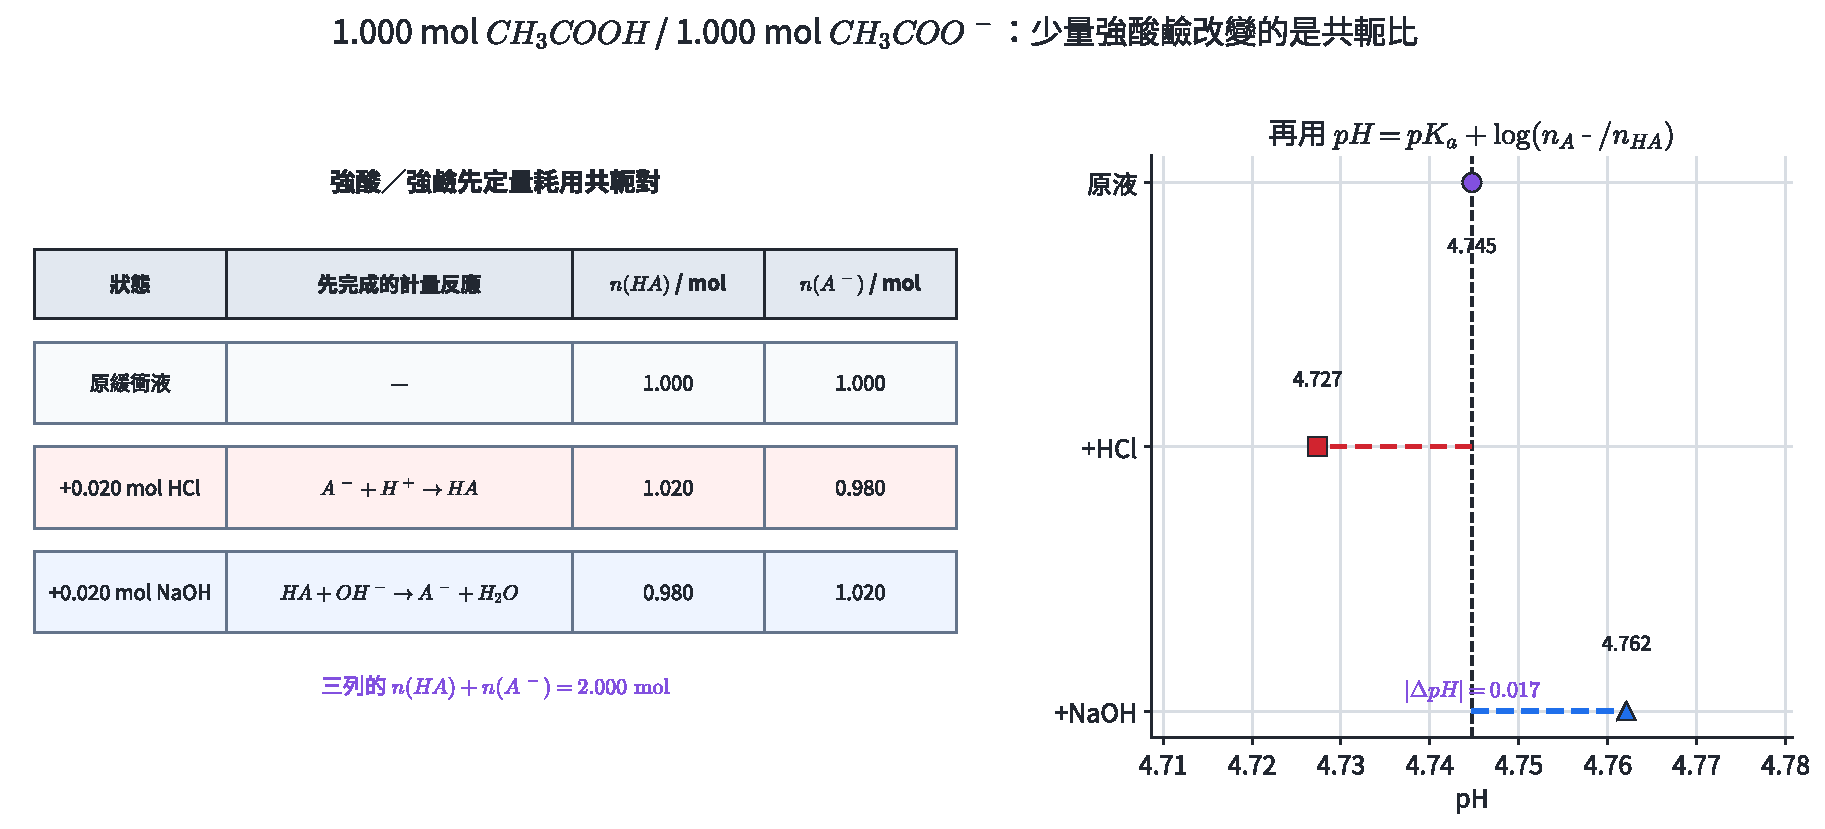
\includegraphics[width=0.97\linewidth,height=\textheight,keepaspectratio,alt={圖 9｜左圖先用計量反應帳算出加入 HCl 或 NaOH 後的 HA、A− 莫耳數；右圖再將共軛比轉成 pH，兩種擾動的 pH 變化量均約 0.017。}]{assets/選化III-2-緩衝液加入酸鹼.pdf}
\caption{圖 9｜左圖先用計量反應帳算出加入 HCl 或 NaOH 後的 HA、A− 莫耳數；右圖再將共軛比轉成 pH，兩種擾動的 pH 變化量均約 0.017。}
\end{figure}

\subsection{10.2 Henderson--Hasselbalch 關係}\label{hendersonhasselbalch-ux95dcux4fc2}

由

\[
K_a=\frac{[H^+][A^-]}{[HA]}
\]

移項並取負對數：

\[
[H^+]=K_a\frac{[HA]}{[A^-]},
\]

\[
pH=pK_a+\log\frac{[A^-]}{[HA]}.
\]

弱鹼緩衝系可寫為

\[
pOH=pK_b+\log\frac{[BH^+]}{[B]}.
\]

混合溶液含強酸或強鹼時，先完成定量反應，再把剩餘弱物種代入比例式。

\subsection{10.3 範圍與容量}\label{ux7bc4ux570dux8207ux5bb9ux91cf}

當 \(0.1\le[A^-]/[HA]\le10\)，通常有

\[
pK_a-1\le pH\le pK_a+1.
\]

目標 pH 決定共軛比；共軛物種總濃度決定可吸收多少外加酸鹼。兩者接近等量時，對酸與鹼的容量較均衡。

\begin{figure}
\centering
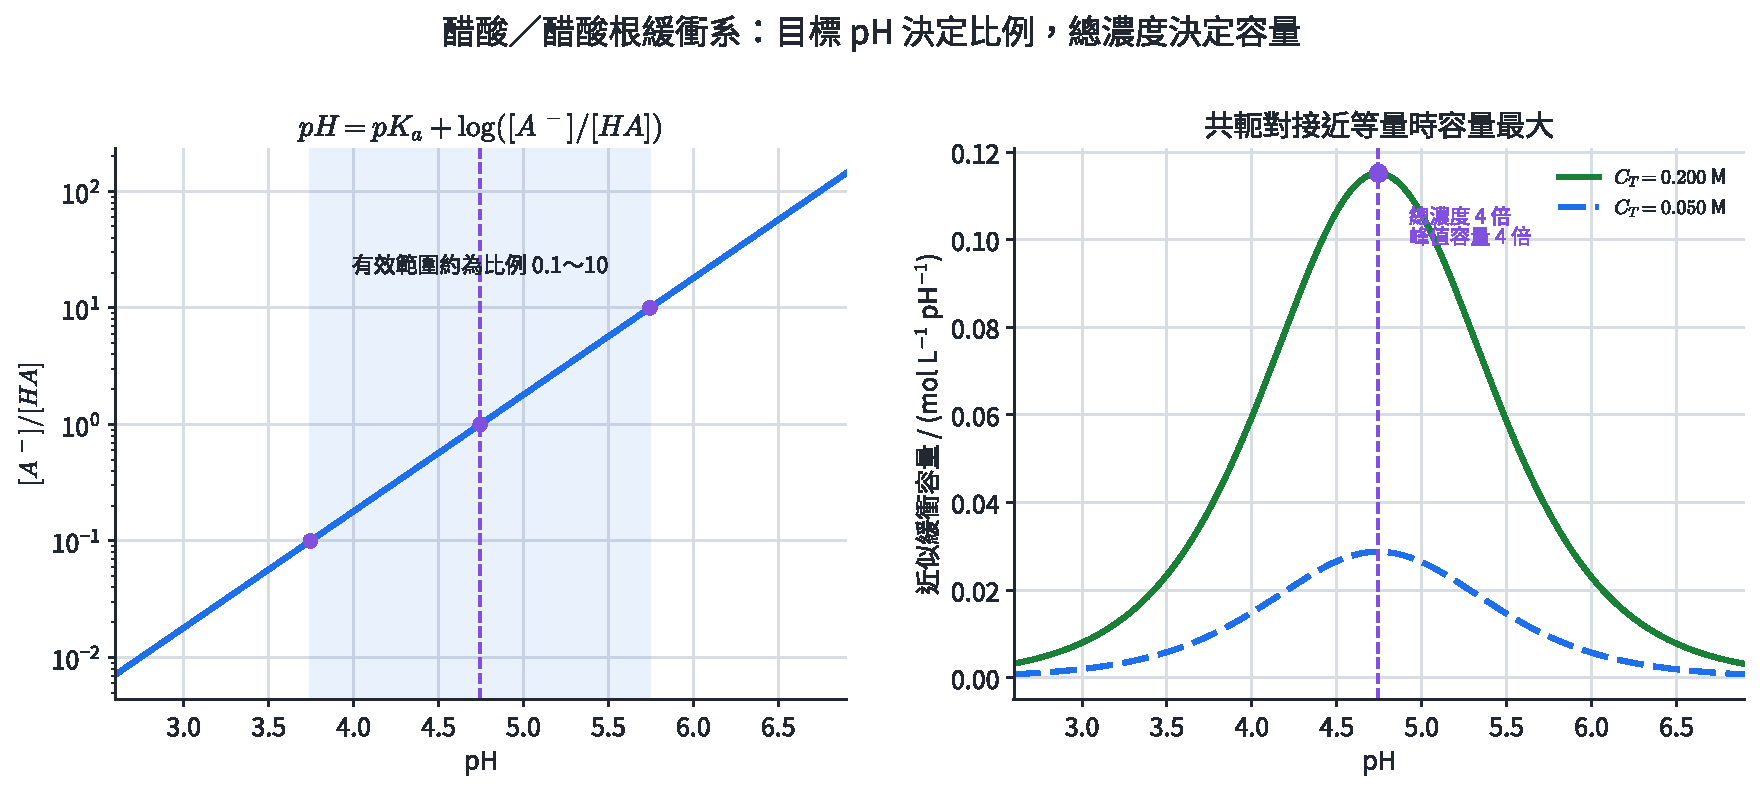
\includegraphics[width=0.96\linewidth,height=\textheight,keepaspectratio,alt={圖 10｜左圖把 pH 轉成共軛鹼／弱酸比例；右圖顯示共軛對在 pH = pKa 時的近似緩衝容量最大，且總濃度增為 4 倍時，峰值容量也增為 4 倍。}]{assets/選化III-2-緩衝比例與容量.pdf}
\caption{圖 10｜左圖把 pH 轉成共軛鹼／弱酸比例；右圖顯示共軛對在 pH = pKa 時的近似緩衝容量最大，且總濃度增為 4 倍時，峰值容量也增為 4 倍。}
\end{figure}

\begin{HandoutWorkedExample}

\subsection{示範 19｜由共軛比求醋酸緩衝液 pH}\label{ux793aux7bc4-19ux7531ux5171ux8edbux6bd4ux6c42ux918bux9178ux7de9ux885dux6db2-ph}

一溶液含 \(0.200\ \mathrm M\) \(CH_3COOH\) 與
\(0.100\ \mathrm M\) \(CH_3COO^-\)，\(K_a=1.8\times10^{-5}\)：

\[
pK_a=4.745.
\]

\[
pH=4.745+\log\frac{0.100}{0.200}
=4.745-0.301
=4.444.
\]

酸量是共軛鹼的兩倍，所以 pH 比 \(pK_a\) 低 \(0.301\)。

\end{HandoutWorkedExample}

\begin{HandoutWorkedExample}

\subsection{示範 20｜部分中和配製氨緩衝液}\label{ux793aux7bc4-20ux90e8ux5206ux4e2dux548cux914dux88fdux6c28ux7de9ux885dux6db2}

混合 \(100.0\) mL \(0.200\ \mathrm M\) \(NH_3\) 與
\(50.0\) mL \(0.200\ \mathrm M\) \(HCl\)：

\[
n(NH_3)=0.0200\ \mathrm{mol},\qquad n(H^+)=0.0100\ \mathrm{mol}.
\]

\[
NH_3+H^+\rightarrow NH_4^+.
\]

反應後 \(NH_3\) 與 \(NH_4^+\) 各 \(0.0100\) mol。\(K_b(NH_3)=1.8\times10^{-5}\)，故

\[
pOH=pK_b+\log\frac{n(NH_4^+)}{n(NH_3)}
=4.745,
\]

\[
pH=9.255.
\]

再加入 \(0.0010\) mol \(HCl\)，新莫耳數為

\[
n(NH_3)=0.0090,\qquad n(NH_4^+)=0.0110.
\]

\[
pOH=4.745+\log\frac{0.0110}{0.0090}=4.832,
\]

\[
pH=9.168.
\]

加入強酸後 pH 下降 \(0.087\)，變化直接來自共軛比。

\end{HandoutWorkedExample}

生物實驗的磷酸鹽緩衝液、藥品與食品製程、發酵槽及 pH 電極校正液都利用此機制。血液 pH 還受到呼吸排出 \(CO_2\)、腎臟調節與蛋白質等多套系統共同控制；單一 Henderson--Hasselbalch 式描述其中一組共軛對。

\subsection{分節練習 10}\label{ux5206ux7bc0ux7df4ux7fd2-10}

\begin{enumerate}
\def\labelenumi{\arabic{enumi}.}
\tightlist
\item
  下列混合均在反應後判斷：

  \begin{enumerate}
  \def\labelenumii{(\alph{enumii})}
  \tightlist
  \item
    等莫耳 \(CH_3COOH\)、\(CH_3COONa\)；\\
  \item
    \(0.010\) mol \(NH_3\)、\(0.004\) mol \(HCl\)；\\
  \item
    等莫耳 \(HCl\)、\(NaOH\)；\\
  \item
    \(0.010\) mol \(NH_4Cl\)、\(0.004\) mol \(NaOH\)。\\
    哪些形成緩衝液？
  \end{enumerate}
\item
  用 \(1.000\) mol 醋酸與 \(NaOH\) 配製 pH \(=5.00\) 的緩衝液。\(K_a=1.8\times10^{-5}\)，求需加入的 \(NaOH\) 莫耳數。
\item
  一緩衝液含 \(0.0500\) mol 醋酸與 \(0.0500\) mol 醋酸根。加入 \(0.0050\) mol \(HCl\) 後求 pH。\(pK_a=4.745\)。
\item
  甲含 \(0.10\ \mathrm M\) \(HA\) 與 \(0.10\ \mathrm M\) \(A^-\)；乙含 \(1.0\ \mathrm M\) \(HA\) 與 \(1.0\ \mathrm M\) \(A^-\)。比較初始 pH 與加入相同少量強酸後的 pH 變化。
\end{enumerate}

\subsection{分節練習 10 解析}\label{ux5206ux7bc0ux7df4ux7fd2-10-ux89e3ux6790}

\begin{enumerate}
\def\labelenumi{\arabic{enumi}.}
\tightlist
\item
  \begin{enumerate}
  \def\labelenumii{(\alph{enumii})}
  \tightlist
  \item
    直接含弱酸與共軛鹼，是緩衝液。(b) \(HCl\) 消耗部分 \(NH_3\)，留下 \(0.006\) mol \(NH_3\) 並生成 \(0.004\) mol \(NH_4^+\)，是緩衝液。(c) 完全中和後只剩強酸強鹼鹽，不是緩衝液。(d) \(OH^-\) 消耗部分 \(NH_4^+\)，生成 \(NH_3\) 且保留 \(NH_4^+\)，是緩衝液。
  \end{enumerate}
\item
  \[
   \frac{[CH_3COO^-]}{[CH_3COOH]}
   =10^{5.00-4.745}=1.80.
   \]
  設加入 \(x\) mol \(NaOH\)，反應後共軛鹼為 \(x\)、醋酸為 \(1.000-x\)：
  \[
   \frac{x}{1.000-x}=1.80.
   \]
  解得 \(x=0.643\ \mathrm{mol}\)。
\item
  \(H^+\) 先把醋酸根轉成醋酸：
  \[
  n(A^-)=0.0450,\qquad n(HA)=0.0550\ \mathrm{mol}.
  \]
  \[
  pH=4.745+\log\frac{0.0450}{0.0550}=4.658.
  \]
\item
  兩杯的共軛比都是 \(1\)，所以初始 pH 均為 \(pK_a\)。乙的兩物種莫耳數是甲的十倍；加入相同少量強酸時，乙的比例改變較小，因此 pH 變化較小、緩衝容量較大。
\end{enumerate}

\section{11. 酸鹼滴定、指示劑與實驗證據}\label{ux9178ux9e7cux6ef4ux5b9aux6307ux793aux5291ux8207ux5be6ux9a57ux8b49ux64da}

\subsection{11.1 當量點的化學計量}\label{ux7576ux91cfux9edeux7684ux5316ux5b78ux8a08ux91cf}

滴定以已知濃度的標準溶液測定未知物。當量點是反應物依化學計量恰好反應的狀態。若一個酸分子在指定滴定中提供 \(a\) 個質子，一個鹼粒子提供 \(b\) 個氫氧根：

\[
C_aV_a a=C_bV_b b.
\]

這是 \(H^+\) 當量與 \(OH^-\) 當量相等，不要求酸、鹼的莫耳數相等。

終點是儀器或指示劑顯示停止滴定的觀測時刻。合適方法使終點落在當量點附近，兩者的體積差形成滴定誤差。

\subsection{11.2 指示劑的平衡}\label{ux6307ux793aux5291ux7684ux5e73ux8861}

酸式指示劑可寫成

\[
HIn\rightleftharpoons H^++In^-.
\]

兩種型態顏色不同：

\[
pH=pK_{a,\mathrm{In}}+\log\frac{[In^-]}{[HIn]}.
\]

人眼通常在兩型比例約從 \(1:10\) 變到 \(10:1\) 的區間看見明顯轉色，因此變色範圍約為 \(pK_{a,\mathrm{In}}\pm1\)。指示劑範圍需落在滴定曲線的陡升或陡降區。

\subsection{11.3 標定、器材與操作}\label{ux6a19ux5b9aux5668ux6750ux8207ux64cdux4f5c}

\(NaOH\) 固體與溶液會吸收空氣中的水與 \(CO_2\)，配製後以純度高、組成穩定的基準物質標定。鄰苯二甲酸氫鉀（KHP）是單質子酸，與 \(OH^-\) 依 \(1:1\) 反應。

\begin{figure}
\centering
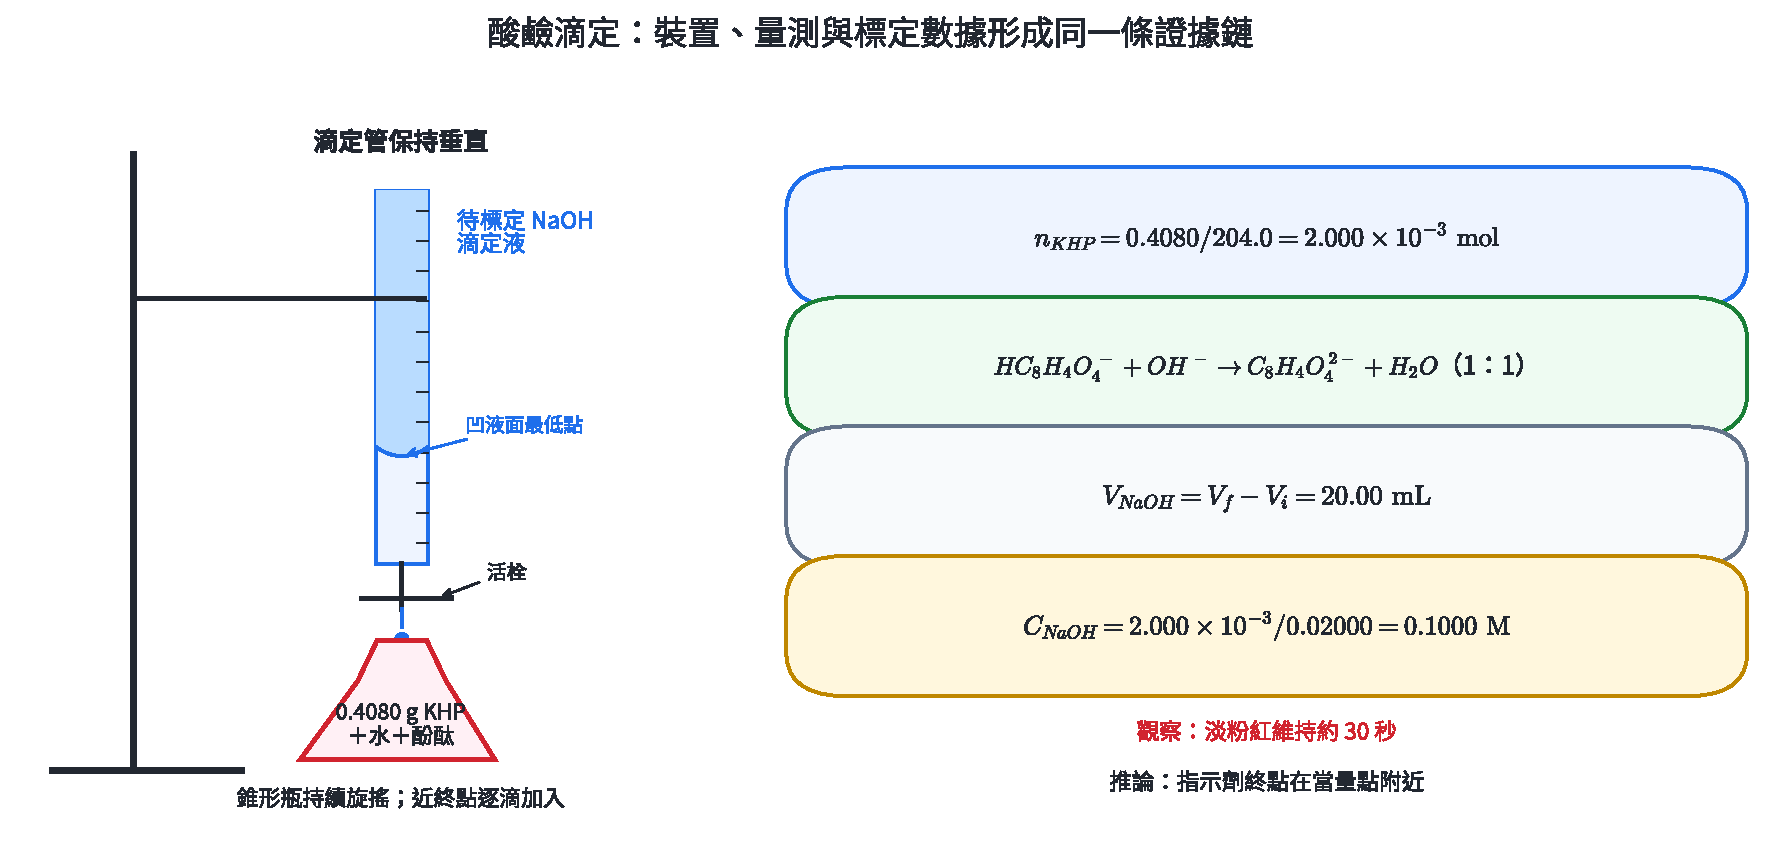
\includegraphics[width=0.97\linewidth,height=\textheight,keepaspectratio,alt={圖 11｜左圖顯示待標定 NaOH 滴定 KHP 的實際裝置與終點操作；右圖以淨離子反應的 1：1 關係、Vf − Vi 與 KHP 質量求得 NaOH 濃度。}]{assets/選化III-2-滴定裝置與數據.pdf}
\caption{圖 11｜左圖顯示待標定 NaOH 滴定 KHP 的實際裝置與終點操作；右圖以淨離子反應的 1：1 關係、Vf − Vi 與 KHP 質量求得 NaOH 濃度。}
\end{figure}

操作的量測邏輯如下：

\begin{enumerate}
\def\labelenumi{\arabic{enumi}.}
\tightlist
\item
  滴定管以滴定液潤洗，排除尖端氣泡，垂直固定後讀初刻度。
\item
  待測液用移液吸管定量移入錐形瓶；錐形瓶可用蒸餾水洗，殘留蒸餾水只改變總體積，不改變待測物莫耳數。
\item
  滴定中持續旋搖；接近終點改成逐滴加入，記錄終刻度。
\item
  重複到取得相近滴定體積，以相近試次平均。
\end{enumerate}

強酸、強鹼具有腐蝕性。操作需穿實驗衣、戴護目鏡與合適手套；漏斗加液後移除，滴定管最高處的加液在安全高度進行。酸、鹼廢液依校內規範分流，經教師指定程序中和或回收；含指示劑、有機物或金屬離子的廢液依成分另行收集。紀錄中的「淡粉紅維持約 30 秒」是觀察；「已到達設定終點」是依指示劑模型作出的推論。

\begin{HandoutWorkedExample}

\subsection{\texorpdfstring{示範 21｜以 KHP 標定 \(NaOH\)}{示範 21｜以 KHP 標定 NaOH}}\label{ux793aux7bc4-21ux4ee5-khp-ux6a19ux5b9a-naoh}

取 \(0.4080\) g KHP，式量 \(204.0\)，滴定需 \(20.00\) mL \(NaOH\)。

\[
n(KHP)=\frac{0.4080}{204.0}=2.000\times10^{-3}\ \mathrm{mol}.
\]

反應比為 \(1:1\)：

\[
n(NaOH)=2.000\times10^{-3}\ \mathrm{mol}.
\]

\[
C_{NaOH}=\frac{2.000\times10^{-3}}{0.02000}
=0.1000\ \mathrm M.
\]

有效數字由 KHP 質量、式量與滴定體積共同限制。

\end{HandoutWorkedExample}

\begin{HandoutWorkedExample}

\subsection{示範 22｜由滴定求食醋重量百分率}\label{ux793aux7bc4-22ux7531ux6ef4ux5b9aux6c42ux98dfux918bux91cdux91cfux767eux5206ux7387}

量取 \(5.00\) mL 食醋，密度為 \(1.01\ \mathrm{g\,mL^{-1}}\)；以 \(0.1000\ \mathrm M\) \(NaOH\) 滴定，平均需 \(41.80\) mL。醋酸為單質子酸：

\[
n(CH_3COOH)=n(NaOH)
=(0.1000)(0.04180)
=4.180\times10^{-3}\ \mathrm{mol}.
\]

以醋酸摩爾質量 \(60.05\ \mathrm{g\,mol^{-1}}\)：

\[
m(CH_3COOH)=(4.180\times10^{-3})(60.05)
=0.2510\ \mathrm g.
\]

食醋樣品質量：

\[
m_{\mathrm{sample}}=(5.00)(1.01)=5.05\ \mathrm g.
\]

\[
w\%=\frac{0.2510}{5.05}\times100\%=4.97\%.
\]

這項結果是樣品中可依 \(1:1\) 與 \(NaOH\) 反應的醋酸當量；其他可滴定酸存在時會一起貢獻。

\end{HandoutWorkedExample}

滴定可用於食醋、制酸劑、水質鹼度與製程藥液。量測結果取決於標準液濃度、取樣代表性、反應選擇性與終點判定；醫療樣品還需使用經驗證的臨床分析方法。

\subsection{分節練習 11}\label{ux5206ux7bc0ux7df4ux7fd2-11}

\begin{enumerate}
\def\labelenumi{\arabic{enumi}.}
\tightlist
\item
  \(15.0\) mL 草酸 \(H_2C_2O_4\) 以 \(0.100\ \mathrm M\) \(NaOH\) 滴定，需 \(48.0\) mL 完全反應。求草酸濃度。
\item
  \(25.00\) mL 未知二質子酸以 \(0.2000\ \mathrm M\) \(NaOH\) 滴定，需 \(30.00\) mL 達第二當量點。求酸濃度。
\item
  某指示劑 \(pK_a=4.80\)。在 pH \(=5.80\) 時求 \([In^-]/[HIn]\)，判斷主要顏色型態。
\item
  同一樣品的滴定體積為 \(24.10\)、\(24.15\)、\(25.20\) mL。指出可先採用的相近試次與平均值，並說明下一步。
\end{enumerate}

\subsection{分節練習 11 解析}\label{ux5206ux7bc0ux7df4ux7fd2-11-ux89e3ux6790}

\begin{enumerate}
\def\labelenumi{\arabic{enumi}.}
\tightlist
\item
  \[
   C_a(0.0150)(2)=(0.100)(0.0480)(1).
   \]
  \(C_a=0.160\ \mathrm M\)。
\item
  \[
   C_a(0.02500)(2)=(0.2000)(0.03000)(1).
   \]
  \(C_a=0.1200\ \mathrm M\)。
\item
  \[
   5.80=4.80+\log\frac{[In^-]}{[HIn]},
   \]
  因此 \([In^-]/[HIn]=10\)，顏色以鹼式 \(In^-\) 為主，正位於常見轉色範圍的高 pH 端。
\item
  \(24.10\)、\(24.15\) mL 相差 \(0.05\) mL，可先取平均 \(24.125\) mL，依器材解析度報為 \(24.13\) mL。\(25.20\) mL 與前兩次差距大，需檢查終點過滴、氣泡、漏液或讀值，再重複滴定取得另一個相近試次。
\end{enumerate}

\section{12. 滴定曲線、半當量點與分區模型}\label{ux6ef4ux5b9aux66f2ux7ddaux534aux7576ux91cfux9edeux8207ux5206ux5340ux6a21ux578b}

\subsection{12.1 滴定曲線的四個計算區域}\label{ux6ef4ux5b9aux66f2ux7ddaux7684ux56dbux500bux8a08ux7b97ux5340ux57df}

滴定曲線以 pH 為縱軸、已加入滴定液體積為橫軸。對強鹼滴定單質子弱酸，可依主要物種分四區：

\begin{enumerate}
\def\labelenumi{\arabic{enumi}.}
\tightlist
\item
  \textbf{起點：}只有弱酸，使用 \(K_a\) 平衡。
\item
  \textbf{當量點前：}中和後同時有 \(HA/A^-\)，使用緩衝比。
\item
  \textbf{當量點：}弱酸轉成 \(A^-\)，使用鹽類水解。
\item
  \textbf{當量點後：}過量強鹼決定 \([OH^-]\)。
\end{enumerate}

\begin{figure}
\centering
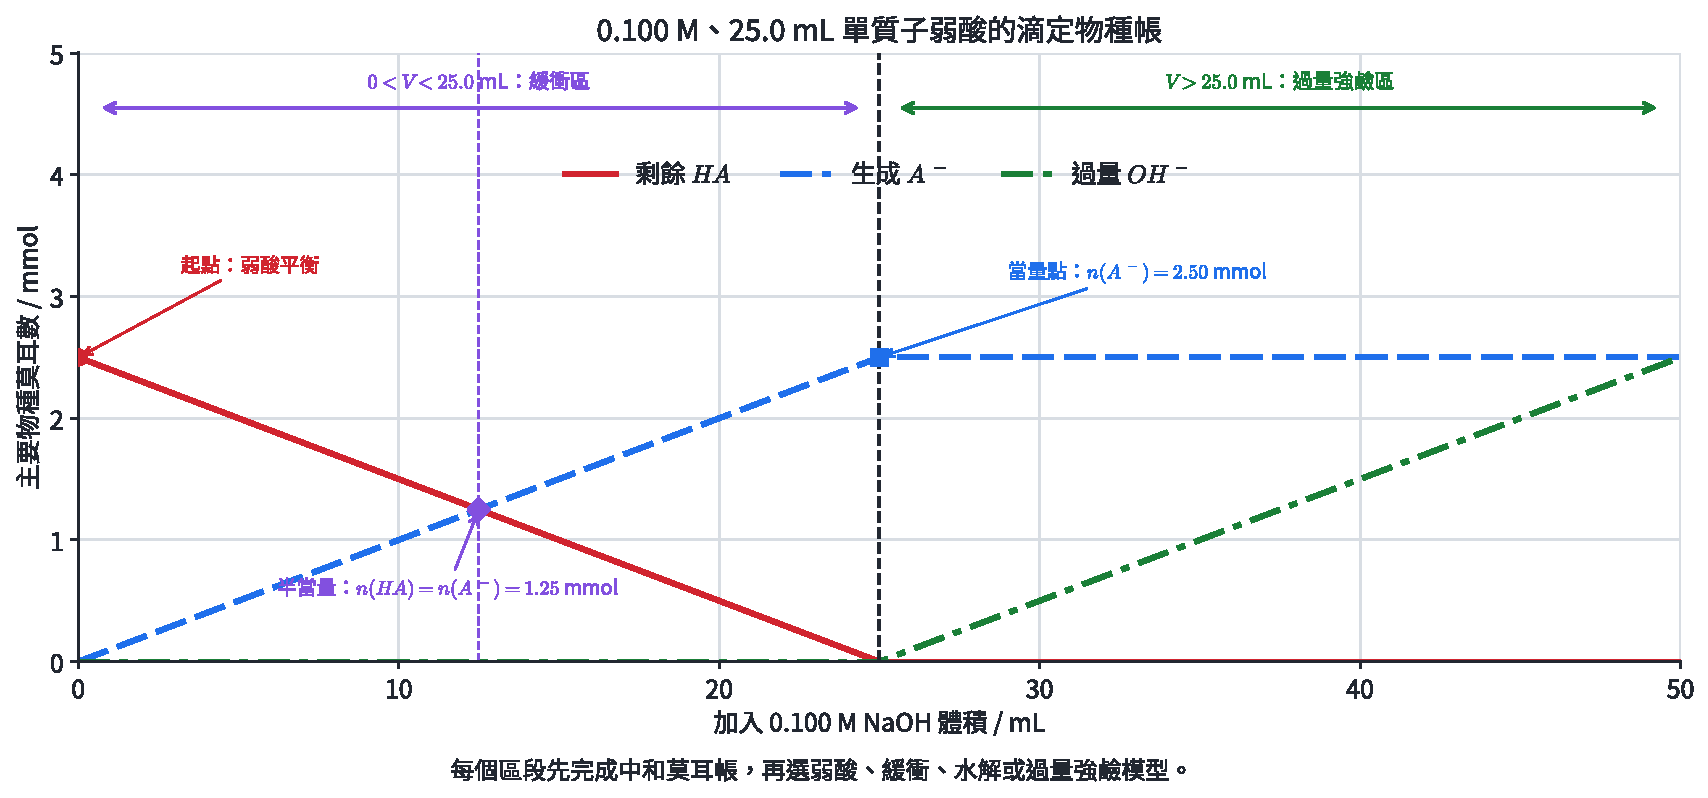
\includegraphics[width=0.97\linewidth,height=\textheight,keepaspectratio,alt={圖 12｜弱酸滴定的三條莫耳數曲線；點標出起點、半當量與當量狀態，上方區間線把 0 \textless{} V \textless{} 25.0 mL 的緩衝區與 V \textgreater{} 25.0 mL 的過量強鹼區分開。}]{assets/選化III-2-弱酸滴定分區與物種.pdf}
\caption{圖 12｜弱酸滴定的三條莫耳數曲線；點標出起點、半當量與當量狀態，上方區間線把 0 \textless{} V \textless{} 25.0 mL 的緩衝區與 V \textgreater{} 25.0 mL 的過量強鹼區分開。}
\end{figure}

半當量點有

\[
n(HA)=n(A^-),
\]

因此

\[
pH=pK_a.
\]

強酸滴定弱鹼的對應關係為半當量點 \(pOH=pK_b\)，也可寫成 \(pH=pK_a(BH^+)\)。

\subsection{12.2 當量體積與當量點 pH}\label{ux7576ux91cfux9ad4ux7a4dux8207ux7576ux91cfux9ede-ph}

同濃度、同體積、同質子數的強酸與弱酸，需要相同體積的強鹼達當量點；酸的強弱改變起點、緩衝區與當量點 pH，並不改變總可中和莫耳數。

\begin{itemize}
\tightlist
\item
  強酸－強鹼在 \(25\,^\circ\mathrm C\) 的當量點近似 pH \(7\)。
\item
  弱酸－強鹼的當量點含共軛鹼，pH 大於 \(7\)。
\item
  弱鹼－強酸的當量點含共軛酸，pH 小於 \(7\)。
\end{itemize}

\begin{figure}
\centering
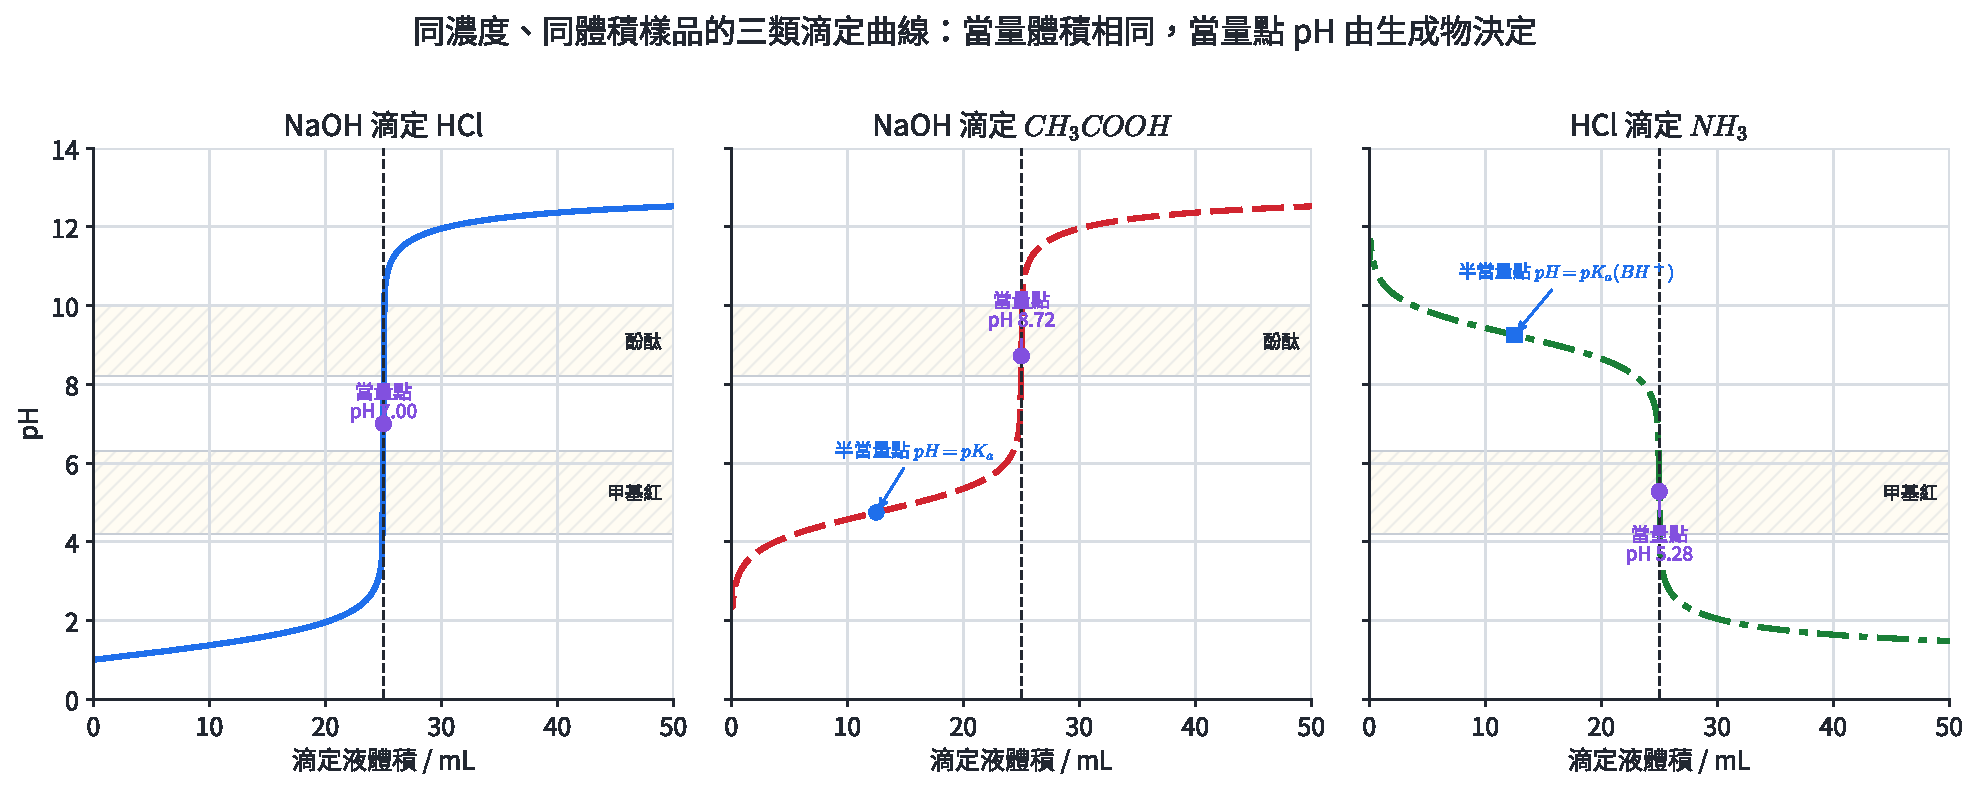
\includegraphics[width=0.99\linewidth,height=\textheight,keepaspectratio,alt={圖 13｜三條曲線均由濃度與莫耳數模型數值生成，當量體積皆為 25.0 mL；點標出當量點與兩個半當量點，斜線帶是甲基紅或酚酞的變色範圍。}]{assets/選化III-2-三類滴定曲線.pdf}
\caption{圖 13｜三條曲線均由濃度與莫耳數模型數值生成，當量體積皆為 25.0 mL；點標出當量點與兩個半當量點，斜線帶是甲基紅或酚酞的變色範圍。}
\end{figure}

指示劑需在當量點附近的陡變區轉色。弱酸－強鹼通常選酚酞；弱鹼－強酸通常選甲基紅。強酸－強鹼陡變範圍較寬，多種範圍落在陡變區的指示劑都可使用。

\begin{HandoutWorkedExample}

\subsection{示範 23｜弱酸－強鹼曲線的四個特徵點}\label{ux793aux7bc4-23ux5f31ux9178ux5f37ux9e7cux66f2ux7ddaux7684ux56dbux500bux7279ux5fb5ux9ede}

以 \(0.100\ \mathrm M\) \(NaOH\) 滴定 \(25.00\) mL
\(0.100\ \mathrm M\) \(CH_3COOH\)，\(K_a=1.8\times10^{-5}\)。

初始酸莫耳數：

\[
n_0=(0.100)(0.02500)=2.500\times10^{-3}\ \mathrm{mol}.
\]

當量體積：

\[
V_{\mathrm{eq}}=\frac{2.500\times10^{-3}}{0.100}
=25.00\ \mathrm{mL}.
\]

\textbf{起點，\(V_b=0\)：}

解 \(x^2/(0.100-x)=1.8\times10^{-5}\) 得
\([H^+]=1.33\times10^{-3}\ \mathrm M\)，pH \(=2.875\)。

\textbf{半當量點，\(V_b=12.50\) mL：}

\[
pH=pK_a=4.745.
\]

\textbf{當量點，\(V_b=25.00\) mL：}

醋酸根濃度

\[
C=\frac{2.500\times10^{-3}}{0.05000}
=0.0500\ \mathrm M.
\]

\[
K_b=\frac{10^{-14}}{1.8\times10^{-5}}
=5.56\times10^{-10}.
\]

水解得 \([OH^-]=5.27\times10^{-6}\ \mathrm M\)，所以 pH \(=8.722\)。

\textbf{過量鹼，\(V_b=30.00\) mL：}

\[
n_{\mathrm{excess}}(OH^-)
=(0.100)(0.03000)-2.500\times10^{-3}
=5.00\times10^{-4}\ \mathrm{mol}.
\]

\[
[OH^-]=\frac{5.00\times10^{-4}}{0.05500}
=9.09\times10^{-3}\ \mathrm M,
\]

所以 pH \(=11.959\)。

\end{HandoutWorkedExample}

\begin{HandoutWorkedExample}

\subsection{示範 24｜弱鹼－強酸的半當量與當量點}\label{ux793aux7bc4-24ux5f31ux9e7cux5f37ux9178ux7684ux534aux7576ux91cfux8207ux7576ux91cfux9ede}

以 \(0.100\ \mathrm M\) \(HCl\) 滴定 \(25.00\) mL
\(0.100\ \mathrm M\) \(NH_3\)，\(K_b=1.8\times10^{-5}\)。當量體積也是 \(25.00\) mL。

半當量點時 \(n(NH_3)=n(NH_4^+)\)：

\[
pOH=pK_b=4.745,
\]

\[
pH=9.255.
\]

當量點只剩 \(0.0500\ \mathrm M\) \(NH_4^+\)：

\[
K_a(NH_4^+)=5.56\times10^{-10}.
\]

水解得 \([H^+]=5.27\times10^{-6}\ \mathrm M\)，所以 pH \(=5.278\)。甲基紅的變色範圍 \(4.2\)～\(6.3\) 落在當量點附近陡降區，可作此滴定的指示劑。

\end{HandoutWorkedExample}

滴定曲線可同時給出濃度、\(pK_a\)、緩衝範圍與當量點。真實曲線受電極校正、溫度、離子強度、混合時間與多重酸鹼平衡影響；資料點不足時，以陡變區間估計當量體積並報告解析度。

\subsection{分節練習 12}\label{ux5206ux7bc0ux7df4ux7fd2-12}

\begin{enumerate}
\def\labelenumi{\arabic{enumi}.}
\tightlist
\item
  以 \(0.100\ \mathrm M\) \(NaOH\) 滴定 \(25.00\) mL \(0.100\ \mathrm M\) \(HCl\)。求加入 \(0\)、\(12.50\)、\(25.00\)、\(30.00\) mL 時的 pH。
\item
  甲基橙、甲基紅、酚酞的變色範圍依序為 \(3.1\)～\(4.4\)、\(4.2\)～\(6.3\)、\(8.2\)～\(10.0\)。分別為強鹼滴定醋酸、強酸滴定氨選擇合適指示劑。
\item
  \(30.0\) mL 果醋以 \(0.100\ \mathrm M\) \(NaOH\) 滴定，量得資料：\\
  \(V_b/\mathrm{mL}=0,5,10,15,20,25,30,35,40\)；\\
  pH \(=3.0,4.3,4.7,5.0,5.3,5.7,8.8,11.9,12.2\)。\\
  估計當量體積、醋酸濃度、半當量點 \(pK_a\) 與緩衝區。
\item
  同體積、同濃度的 \(HCl\) 與 \(CH_3COOH\) 分別用同一 \(NaOH\) 滴定。比較當量體積、起始 pH、當量點 pH 與可見緩衝區。
\end{enumerate}

\subsection{分節練習 12 解析}\label{ux5206ux7bc0ux7df4ux7fd2-12-ux89e3ux6790}

\begin{enumerate}
\def\labelenumi{\arabic{enumi}.}
\tightlist
\item
  起點 \([H^+]=0.100\ \mathrm M\)，pH \(=1.000\)。加入 \(12.50\) mL：
  \[
  [H^+]=\frac{(0.100)(0.02500)-(0.100)(0.01250)}
  {0.03750}
  =0.03333\ \mathrm M,
  \]
  pH \(=1.477\)。加入 \(25.00\) mL 達強酸強鹼當量點，pH \(=7.000\)。加入 \(30.00\) mL：
  \[
  [OH^-]=\frac{(0.100)(0.03000)-(0.100)(0.02500)}
  {0.05500}
  =9.09\times10^{-3}\ \mathrm M,
  \]
  pH \(=11.959\)。
\item
  強鹼滴定醋酸的當量點呈鹼性，選酚酞；強酸滴定氨的當量點呈酸性，選甲基紅。
\item
  最大陡升在 \(25\)～\(30\) mL，當量體積約 \(30.0\) mL：
  \[
  C_{\mathrm{acid}}(0.0300)=(0.100)(0.0300),
  \]
  所以醋酸濃度約 \(0.100\ \mathrm M\)。半當量體積 \(15.0\) mL，故 \(pK_a\approx5.0\)。約 \(5\)～\(25\) mL 同時有醋酸與醋酸根，可辨認為緩衝區；實際邊界由資料解析度決定。
\item
  兩杯可中和的酸莫耳數相同，所以當量體積相同。\(HCl\) 起始 pH 較低，強酸－強鹼當量點在 \(25\,^\circ\mathrm C\) 約為 \(7\)；醋酸起始 pH 較高，當量點因醋酸根水解而大於 \(7\)。醋酸滴定在當量點前有明顯緩衝區，鹽酸滴定沒有弱酸／共軛鹼緩衝區。
\end{enumerate}

\section{13. 章末分層題}\label{ux7ae0ux672bux5206ux5c64ux984c}

\subsection{基礎題}\label{ux57faux790eux984c}

\begin{enumerate}
\def\labelenumi{\arabic{enumi}.}
\item
  寫出下列物質的名稱，並指出可解離的酸性氫或氫氧根數目：\(HClO_2\)、\(HCN(aq)\)、\(Fe(OH)_3\)、\(H_3PO_3\)。已知 \(H_3PO_3\) 的結構可寫成 \(HPO(OH)_2\)。
\item
  對反應
  \[
  H_2PO_4^-+NH_3\rightleftharpoons HPO_4^{2-}+NH_4^+
  \]
  指出兩組共軛酸鹼對，並寫出正向反應中酸與鹼的角色。
\item
  某溫度下 \(K_w=2.50\times10^{-14}\)。求中性水的 pH，並判斷同溫下 pH \(=7.00\) 的溶液呈酸性、中性或鹼性。
\item
  \(0.0500\ \mathrm M\) 一元弱酸 \(HA\) 的 \(K_a=2.00\times10^{-5}\)。以二次方程求 \([H^+]\)、pH 與解離百分率。
\item
  某弱酸的 \(K_a=2.00\times10^{-5}\)。求其共軛鹼的 \(K_b\)，溫度取 \(25\,^\circ\mathrm C\)。
\item
  將下列鹽依組成分為正鹽、酸式鹽、鹼式鹽或複鹽：\(NaH_2PO_4\)、\(NaH_2PO_2\)、\(Ca(OH)Cl\)、\(KAl(SO_4)_2\)。已知 \(H_3PO_2\) 的結構為 \(HOPH_2\)。
\end{enumerate}

\subsection{核心題}\label{ux6838ux5fc3ux984c}

\begin{enumerate}
\def\labelenumi{\arabic{enumi}.}
\setcounter{enumi}{6}
\item
  \(0.200\ \mathrm M\) 甲胺 \(CH_3NH_2\) 的 \(K_b=4.40\times10^{-4}\)。以二次方程求 \([OH^-]\)、pH 與解離百分率。
\item
  將 \(0.100\ \mathrm M\) \(HA\) 與 \(0.100\ \mathrm M\) \(NaA\) 配成溶液，體積變化已計入所列濃度，\(K_a(HA)=1.00\times10^{-5}\)。求 pH，並說明同離子如何改變 \(HA\) 的解離。
\item
  二質子酸 \(H_2A\) 的 \(pK_{a1}=3.00\)、\(pK_{a2}=7.00\)。判斷 pH \(=5.00\) 時主要物種，並指出哪兩個 pH 分別使 \([H_2A]=[HA^-]\)、\([HA^-]=[A^{2-}]\)。
\item
  求 \(0.100\ \mathrm M\) \(NH_4Cl\) 的 pH。已知 \(K_b(NH_3)=1.80\times10^{-5}\)，溫度為 \(25\,^\circ\mathrm C\)。
\item
  一杯緩衝液含 \(0.0300\) mol \(HA\) 與 \(0.0200\) mol \(A^-\)，\(pK_a=4.80\)。求起始 pH；再加入 \(0.00500\) mol \(HCl\)，忽略體積變化，求新 pH。
\item
  同體積、同濃度的一元強酸與一元弱酸分別以同一濃度強鹼滴定。比較兩條曲線的起始 pH、當量體積、當量點 pH 與緩衝區；再說明弱酸－強鹼滴定選用酚酞的依據。
\end{enumerate}

\subsection{跨節整合題}\label{ux8de8ux7bc0ux6574ux5408ux984c}

\begin{enumerate}
\def\labelenumi{\arabic{enumi}.}
\setcounter{enumi}{12}
\tightlist
\item
  取 \(25.00\) mL 未知一元弱酸 \(HA\)，以 \(0.1000\ \mathrm M\) \(NaOH\) 滴定，當量體積為 \(20.00\) mL；起始 pH 為 \(2.900\)。

  \begin{enumerate}
  \def\labelenumii{\arabic{enumii}.}
  \tightlist
  \item
    求原酸濃度。
  \item
    求 \(K_a\) 與 \(pK_a\)。
  \item
    求半當量點 pH。
  \item
    求當量點 pH，溫度取 \(25\,^\circ\mathrm C\)。
  \item
    甲基橙範圍為 \(3.1\)～\(4.4\)，酚酞範圍為 \(8.2\)～\(10.0\)；選出較合適的指示劑。
  \end{enumerate}
\item
  要配製總量為 \(0.200\) mol 的磷酸鹽緩衝液，使 pH \(=7.40\)。選用 \(H_2PO_4^-/HPO_4^{2-}\)，其 \(pK_{a2}=7.21\)。

  \begin{enumerate}
  \def\labelenumii{\arabic{enumii}.}
  \tightlist
  \item
    求兩物種各需多少 mol。
  \item
    若加入 \(0.0100\) mol \(HCl\)，忽略體積變化，求新 pH。
  \item
    以質子轉移方程說明緩衝作用。
  \end{enumerate}
\item
  \(100.0\) mL 溶液含 \(0.0100\) mol 二質子酸 \(H_2A\)，以 \(0.1000\ \mathrm M\) \(NaOH\) 滴定。已知 \(K_{a1}=1.0\times10^{-3}\)、\(K_{a2}=1.0\times10^{-7}\)。

  \begin{enumerate}
  \def\labelenumii{\arabic{enumii}.}
  \tightlist
  \item
    求第一、第二當量體積。
  \item
    估算第一當量點 pH。
  \item
    求加入 \(150.0\) mL \(NaOH\) 時的 pH。
  \item
    求第二當量點 pH，溫度取 \(25\,^\circ\mathrm C\)。
  \end{enumerate}
\item
  以鄰苯二甲酸氫鉀（KHP，式量 \(204.22\ \mathrm{g\,mol^{-1}}\)）標定 \(NaOH\)。稱取 \(0.5100\) g KHP，三次滴定體積為 \(24.92\)、\(24.96\)、\(25.60\) mL。另取 \(5.00\) mL 食醋，密度 \(1.005\ \mathrm{g\,mL^{-1}}\)，以標定後的 \(NaOH\) 滴定，兩次體積為 \(41.30\)、\(41.36\) mL；醋酸式量為 \(60.05\ \mathrm{g\,mol^{-1}}\)。

  \begin{enumerate}
  \def\labelenumii{\arabic{enumii}.}
  \tightlist
  \item
    辨認標定資料中的離群值，並由相符的兩次數據求 \(NaOH\) 濃度。
  \item
    求食醋中醋酸的質量百分率。
  \item
    寫出一項終點觀察、一項由觀察得到的推論，以及兩項必要的實驗安全或品質控制措施。
  \end{enumerate}
\end{enumerate}

\section{14. 章末題完整解析}\label{ux7ae0ux672bux984cux5b8cux6574ux89e3ux6790}

\subsection{第 1 題}\label{ux7b2c-1-ux984c}

\begin{itemize}
\tightlist
\item
  \(HClO_2\) 為亞氯酸，結構中的一個 \(O-H\) 可提供 \(H^+\)，屬一元酸。
\item
  \(HCN(aq)\) 為氫氰酸，可提供一個 \(H^+\)，屬一元酸。
\item
  \(Fe(OH)_3\) 為氫氧化鐵（或氫氧化鐵(III)），每個式量含三個 \(OH^-\)。
\item
  \(H_3PO_3=HPO(OH)_2\) 為亞磷酸；兩個 \(O-H\) 上的氫可解離，\(P-H\) 上的氫保留在陰離子中，所以是二元酸。
\end{itemize}

名稱提供化學式的組成資訊；判斷酸的元數時還要辨認氫所連接的原子。

\subsection{第 2 題}\label{ux7b2c-2-ux984c}

正向反應中，\(H_2PO_4^-\) 把一個質子交給 \(NH_3\)：

\[
\underbrace{H_2PO_4^-}_{\text{酸}}+
\underbrace{NH_3}_{\text{鹼}}
\rightleftharpoons
\underbrace{HPO_4^{2-}}_{\text{共軛鹼}}+
\underbrace{NH_4^+}_{\text{共軛酸}}.
\]

兩組共軛酸鹼對為 \(H_2PO_4^-/HPO_4^{2-}\) 與 \(NH_4^+/NH_3\)，每組只差一個 \(H^+\)。

\subsection{第 3 題}\label{ux7b2c-3-ux984c}

中性條件為 \([H^+]=[OH^-]\)，所以

\[
[H^+]=\sqrt{K_w}=\sqrt{2.50\times10^{-14}}
=1.58\times10^{-7}\ \mathrm M.
\]

\[
pH_{\mathrm{neutral}}=-\log(1.58\times10^{-7})=6.801.
\]

同溫下 pH \(=7.00\) 表示 \([H^+]=1.00\times10^{-7}\ \mathrm M\)，小於中性水的 \([H^+]\)，因此溶液呈鹼性。

\subsection{第 4 題}\label{ux7b2c-4-ux984c}

令 \(HA\) 解離 \(x\ \mathrm M\)：

\[
K_a=\frac{x^2}{0.0500-x}=2.00\times10^{-5}.
\]

整理得

\[
x^2+(2.00\times10^{-5})x-(1.00\times10^{-6})=0.
\]

取正根：

\[
x=9.90\times10^{-4}\ \mathrm M=[H^+].
\]

\[
pH=-\log(9.90\times10^{-4})=3.004,
\]

\[
\text{解離百分率}=\frac{9.90\times10^{-4}}{0.0500}\times100\%
=1.98\%.
\]

\subsection{第 5 題}\label{ux7b2c-5-ux984c}

共軛酸鹼對在同一溫度滿足 \(K_aK_b=K_w\)：

\[
K_b=\frac{1.00\times10^{-14}}{2.00\times10^{-5}}
=5.00\times10^{-10}.
\]

\subsection{第 6 題}\label{ux7b2c-6-ux984c}

\begin{itemize}
\tightlist
\item
  \(NaH_2PO_4\) 中仍有可再解離的酸性氫，屬酸式鹽。
\item
  \(NaH_2PO_2\) 由一元酸 \(H_3PO_2=HOPH_2\) 形成；唯一可解離的 \(O-H\) 已被 \(Na^+\) 取代，屬正鹽。
\item
  \(Ca(OH)Cl\) 的組成仍含 \(OH^-\)，屬鹼式鹽。
\item
  \(KAl(SO_4)_2\) 含兩種陽離子 \(K^+\)、\(Al^{3+}\)，屬複鹽。
\end{itemize}

這個分類描述組成。溶液酸鹼性需再由離子水解判斷。

\subsection{第 7 題}\label{ux7b2c-7-ux984c}

以 \(B\) 表示甲胺，令其與水反應產生 \(x\ \mathrm M\) \(OH^-\)：

\[
K_b=\frac{x^2}{0.200-x}=4.40\times10^{-4}.
\]

\[
x^2+(4.40\times10^{-4})x-(8.80\times10^{-5})=0.
\]

取正根得

\[
[OH^-]=x=9.16\times10^{-3}\ \mathrm M.
\]

\[
pOH=2.038,\qquad pH=14.000-2.038=11.962.
\]

\[
\text{解離百分率}=\frac{9.16\times10^{-3}}{0.200}\times100\%
=4.58\%.
\]

\subsection{第 8 題}\label{ux7b2c-8-ux984c}

此溶液同時含 \(HA\) 與 \(A^-\)，以濃度比寫成

\[
pH=pK_a+\log\frac{[A^-]}{[HA]}.
\]

因 \([A^-]=[HA]=0.100\ \mathrm M\)，

\[
pH=pK_a=-\log(1.00\times10^{-5})=5.000.
\]

外加 \(A^-\) 使平衡
\(HA\rightleftharpoons H^++A^-\)
朝 \(HA\) 移動，\(HA\) 的解離量因而降低。由完整平衡式求得的修正量相對於 \(0.100\ \mathrm M\) 很小，濃度比近似成立。

\subsection{第 9 題}\label{ux7b2c-9-ux984c}

在 pH \(=5.00\) 時，

\[
pH-pK_{a1}=2.00,\qquad pK_{a2}-pH=2.00.
\]

因此 \(HA^-\) 分別比 \(H_2A\) 與 \(A^{2-}\) 約多 \(10^2\) 倍，是主要物種。由 Henderson--Hasselbalch 關係：

\[
[H_2A]=[HA^-]\quad\text{於}\quad pH=pK_{a1}=3.00,
\]

\[
[HA^-]=[A^{2-}]\quad\text{於}\quad pH=pK_{a2}=7.00.
\]

\subsection{第 10 題}\label{ux7b2c-10-ux984c}

\(NH_4Cl\) 完全解離，\(Cl^-\) 對此模型的 pH 貢獻可忽略；\(NH_4^+\) 為弱酸：

\[
K_a(NH_4^+)=\frac{K_w}{K_b(NH_3)}
=\frac{1.00\times10^{-14}}{1.80\times10^{-5}}
=5.56\times10^{-10}.
\]

令水解產生 \(x\ \mathrm M\) \(H^+\)：

\[
K_a=\frac{x^2}{0.100-x}.
\]

解得 \(x=7.45\times10^{-6}\ \mathrm M\)，所以

\[
pH=5.128.
\]

\subsection{第 11 題}\label{ux7b2c-11-ux984c}

起始緩衝液：

\[
pH=4.80+\log\frac{0.0200}{0.0300}=4.624.
\]

加入的強酸先與共軛鹼定量反應：

\[
A^-+H^+\rightarrow HA.
\]

反應後

\[
n(A^-)=0.0200-0.00500=0.0150\ \mathrm{mol},
\]

\[
n(HA)=0.0300+0.00500=0.0350\ \mathrm{mol}.
\]

同一總體積下可用莫耳數比：

\[
pH=4.80+\log\frac{0.0150}{0.0350}=4.432.
\]

\subsection{第 12 題}\label{ux7b2c-12-ux984c}

兩杯酸的體積、濃度與元數相同，可中和的酸莫耳數相同，所以當量體積相同。強酸幾乎完全解離，起始 pH 較低；弱酸只部分解離，起始 pH 較高。

強酸－強鹼在 \(25\,^\circ\mathrm C\) 的當量點約為 pH \(7\)。弱酸－強鹼的當量點含共軛鹼，共軛鹼水解產生 \(OH^-\)，所以當量點 pH 大於 \(7\)。弱酸曲線在當量點前同時含 \(HA\) 與 \(A^-\)，形成緩衝區；強酸曲線沒有這組弱酸／共軛鹼平衡。

酚酞的變色範圍 \(8.2\)～\(10.0\) 落在弱酸－強鹼當量點附近的陡升區，少量滴定劑造成的終點誤差較小，因此適合。

\subsection{第 13 題}\label{ux7b2c-13-ux984c}

當量點的物質量關係為

\[
n(HA)=n(OH^-)=(0.1000)(0.02000)
=2.000\times10^{-3}\ \mathrm{mol}.
\]

原酸濃度：

\[
C_{HA}=\frac{2.000\times10^{-3}}{0.02500}
=0.08000\ \mathrm M.
\]

起始 pH \(=2.900\)，故

\[
x=[H^+]=10^{-2.900}=1.259\times10^{-3}\ \mathrm M.
\]

\[
K_a=\frac{x^2}{0.08000-x}
=2.013\times10^{-5},
\]

\[
pK_a=4.696.
\]

半當量點 \(n(HA)=n(A^-)\)，所以

\[
pH=pK_a=4.696.
\]

當量點總體積為 \(25.00+20.00=45.00\) mL，

\[
[A^-]=\frac{2.000\times10^{-3}}{0.04500}
=0.04444\ \mathrm M.
\]

\[
K_b(A^-)=\frac{1.00\times10^{-14}}{2.013\times10^{-5}}
=4.968\times10^{-10}.
\]

令水解產生 \(x\ \mathrm M\) \(OH^-\)，由

\[
K_b=\frac{x^2}{0.04444-x}
\]

得 \(x=4.70\times10^{-6}\ \mathrm M\)，

\[
pOH=5.328,\qquad pH=8.672.
\]

酚酞的變色範圍包住當量點附近的陡升區，較合適。

\subsection{第 14 題}\label{ux7b2c-14-ux984c}

令 \(n(H_2PO_4^-)=n_a\)、\(n(HPO_4^{2-})=n_b\)。由

\[
7.40=7.21+\log\frac{n_b}{n_a}
\]

得

\[
\frac{n_b}{n_a}=10^{0.19}=1.549.
\]

再聯立 \(n_a+n_b=0.200\) mol：

\[
n_a=0.0785\ \mathrm{mol},\qquad
n_b=0.1215\ \mathrm{mol}.
\]

加入 \(HCl\) 後發生

\[
HPO_4^{2-}+H^+\rightarrow H_2PO_4^-.
\]

因此

\[
n_b'=0.1215-0.0100=0.1115\ \mathrm{mol},
\]

\[
n_a'=0.0785+0.0100=0.0885\ \mathrm{mol}.
\]

\[
pH'=7.21+\log\frac{0.1115}{0.0885}=7.311.
\]

\(HPO_4^{2-}\) 接受外加的 \(H^+\)，把強酸轉成較弱的 \(H_2PO_4^-\)；因此自由 \([H^+]\) 的增加幅度受限。若加入強鹼，\(H_2PO_4^-\) 會把質子轉移給 \(OH^-\)。

\subsection{第 15 題}\label{ux7b2c-15-ux984c}

每莫耳 \(H_2A\) 可分兩步各中和一莫耳 \(OH^-\)。第一當量點需要 \(0.0100\) mol \(OH^-\)：

\[
V_{mathrm{eq1}}=\frac{0.0100}{0.1000}=0.1000\ \mathrm L
=100.0\ \mathrm{mL}.
\]

第二當量點累計需要 \(0.0200\) mol \(OH^-\)：

\[
V_{mathrm{eq2}}=\frac{0.0200}{0.1000}=200.0\ \mathrm{mL}.
\]

第一當量點主要為兩性物種 \(HA^-\)，在 \(K_{a1}\) 與 \(K_{a2}\) 相差甚大時：

\[
pH\approx\frac{pK_{a1}+pK_{a2}}{2}
=\frac{3.00+7.00}{2}=5.00.
\]

加入 \(150.0\) mL 時位於兩個當量點正中間，\(n(HA^-)=n(A^{2-})\)，所以

\[
pH=pK_{a2}=7.00.
\]

第二當量點總體積為 \(100.0+200.0=300.0\) mL，

\[
[A^{2-}]=\frac{0.0100}{0.3000}=0.03333\ \mathrm M.
\]

\[
K_b(A^{2-})=\frac{K_w}{K_{a2}}=1.0\times10^{-7}.
\]

由 \(K_b=x^2/(0.03333-x)\) 得

\[
[OH^-]=5.77\times10^{-5}\ \mathrm M,
\]

\[
pOH=4.239,\qquad pH=9.761.
\]

\subsection{第 16 題}\label{ux7b2c-16-ux984c}

前兩次體積只差 \(0.04\) mL，第三次比其平均值高約 \(0.66\) mL，故 \(25.60\) mL 是離群值。正式實驗應再重複一次；以相符的兩次先求暫定濃度：

\[
\overline V=\frac{24.92+24.96}{2}=24.94\ \mathrm{mL}.
\]

KHP 與 \(NaOH\) 以 \(1:1\) 反應：

\[
n(\mathrm{KHP})=\frac{0.5100}{204.22}
=2.4973\times10^{-3}\ \mathrm{mol}.
\]

\[
C(\mathrm{NaOH})=
\frac{2.4973\times10^{-3}}{0.02494}
=0.10013\ \mathrm M.
\]

食醋滴定的平均體積為

\[
\overline V=\frac{41.30+41.36}{2}=41.33\ \mathrm{mL}.
\]

醋酸與 \(NaOH\) 也是 \(1:1\)：

\[
n(CH_3COOH)=(0.10013)(0.04133)
=4.1385\times10^{-3}\ \mathrm{mol}.
\]

\[
m(CH_3COOH)=(4.1385\times10^{-3})(60.05)
=0.24852\ \mathrm g.
\]

食醋樣品質量為

\[
m_{\mathrm{sample}}=(5.00)(1.005)=5.025\ \mathrm g.
\]

\[
\text{醋酸質量百分率}
=\frac{0.24852}{5.025}\times100\%
=4.95\%.
\]

可直接記錄的終點觀察是「溶液出現均勻淡粉紅色，搖晃後維持約 \(30\) s」。由此推論指示劑已進入變色範圍，滴定接近化學計量當量點。品質控制包括以標準物標定會吸水並吸收 \(CO_2\) 的 \(NaOH\)、對離群值補做滴定並只平均相符數據。安全措施包括配戴護目鏡與手套、以滴管接近終點逐滴加入，並依實驗室規定分流酸鹼廢液。

\section{15. 核心整理}\label{ux6838ux5fc3ux6574ux7406}

\begin{enumerate}
\def\labelenumi{\arabic{enumi}.}
\tightlist
\item
  Brønsted--Lowry 酸把 \(H^+\) 轉移給鹼；一組共軛酸鹼只差一個 \(H^+\)。平衡偏向較弱的酸與較弱的鹼。
\item
  水的離子積為 \(K_w=[H^+][OH^-]\)。中性條件是 \([H^+]=[OH^-]\)；中性 pH 隨溫度與 \(K_w\) 改變。
\item
  弱酸、弱鹼以初始量、變化量、平衡量建立濃度表，再代入 \(K_a\) 或 \(K_b\)。近似須以變化量占初濃度的比例驗證。
\item
  共軛酸鹼對滿足 \(K_aK_b=K_w\)。同離子改變平衡濃度，使弱電解質的解離量降低。
\item
  多質子酸分步解離；物料平衡、電荷平衡與各步平衡常數共同決定物種分布。當 pH 等於某一步 \(pK_a\) 時，相鄰兩物種濃度相等。
\item
  鹽的組成分類與鹽溶液酸鹼性是兩個判定。溶液 pH 由離子的水解強弱與濃度決定。
\item
  緩衝液靠弱酸／共軛鹼或弱鹼／共軛酸先消耗少量外加強鹼或強酸。Henderson--Hasselbalch 式使用反應後的濃度比；總量決定容量。
\item
  滴定計算先做定量中和，再依所在區域選擇過量強酸鹼、緩衝平衡、鹽類水解或當量點模型。指示劑變色範圍要落在當量點附近的陡變區。
\item
  滴定資料需同時保存原始體積、相符試次、終點觀察、標定結果與單位。曲線與數據的解析度決定可報告的當量體積精度。
\end{enumerate}


\end{document}
